
\clearpage
\section{Dokumentenablage}
\label{bkm:Ref434830029}\label{bkm:Ref434828324}

\begin{wrapfigure}[13]{l}{6.5cm}   % [x] Wie manche Zeile soll sich um die Grafik "brechen"
  \vspace{-35pt}      % Grundwert war 20; mit 30 schön oben beim Text ausgerichtet
  \begin{center}
    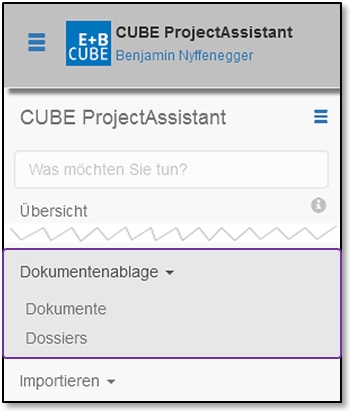
\includegraphics[width=1\linewidth]{../chapters/11_Dokumentenablage/pictures/11_Menu_Dokumentenablage.jpg}
  \end{center}
  \vspace{-20pt}
  \caption{Die Dokumentenablage verwenden}
  \vspace{-10pt}
\end{wrapfigure}

Wählen Sie im Menü links den Punkt 'Dokumentenablage'. Es erscheinen die beiden Unterpunkte 'Dokumente' und 'Dossiers'.

\vspace{\baselineskip}

Die Dokumentenablage dient dazu, Dokumente zu verwalten und gemeinsam zu bearbeiten. Werden Dokumente oder deren Metadaten bearbeitet, erhalten sie im CUBE PA eine neue VersionsnummerD. Einerseits wird mittels dem Aus- und Einchecken sichergestellt, dass ein Dokument nur gerade von einer Person bearbeitet werden kann. Andererseits dient die Versionifizierung der Dokumente dazu, dass sich alle Projektbeteiligten auf eindeutigen Dokumentenversionen beziehen können. 

\vspace{1cm}  

Erfasste, respektive hochgeladene Dokumente können zu Dossiers zusammengefasst werden, welche dann mittels wenigen Klicks heruntergeladen werden können. Deshalb wird in der Anleitung zuerst das Erstellen und Handling eines Dossiers beschrieben.

\vspace{\baselineskip}

Im Anschluss wird die Dokumentenablage detailliert erläutert.

\subsection{Dossiers}
\label{bkm:Ref442544219}\subsubsection{Dossiers erstellen}

Ein Dossier ist ein Satz zusammengehöriger Dokumente. Klassisches Beispiel ist ein Plangenehmigungsdossier oder ein Vorprojekt. Dossiers bieten die Möglichkeit mehrere hochgeladene Dokumente zusammenzufassen, damit sie später gemeinsam in einem ZIP-Archiv heruntergeladen werden können.

\begin{figure}[H]
\center{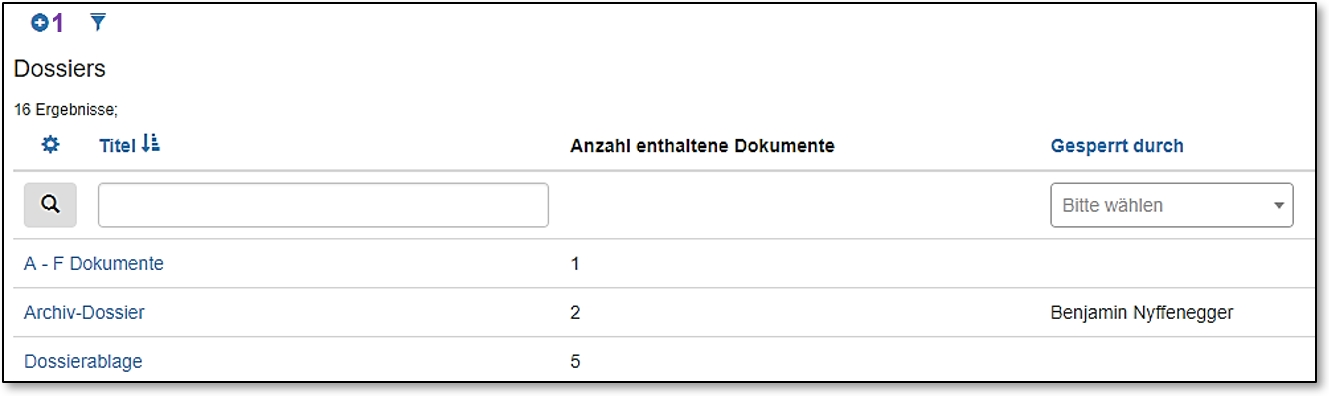
\includegraphics[width=1\linewidth]{../chapters/11_Dokumentenablage/pictures/11-1-1_UebersichtDossiers.jpg}}
\caption{Ein neues Dossier erstellen}
% \label{fig:speciation}
\end{figure}

Um ein neues Dossier zu erstellen, wählen Sie im Menü links unter dem Punkt 'Dokumentenablage' den Unterpunkt 'Dossiers'. Als nächsten Schritt klicken Sie auf das Plussymbol 
\includegraphics[height=12pt]{/Icons/Plussymbol.jpg} \col{(1)}.

\vspace{\baselineskip}

Die Eingabemaske für Dossiers wird geöffnet:

\begin{figure}[H]
\center{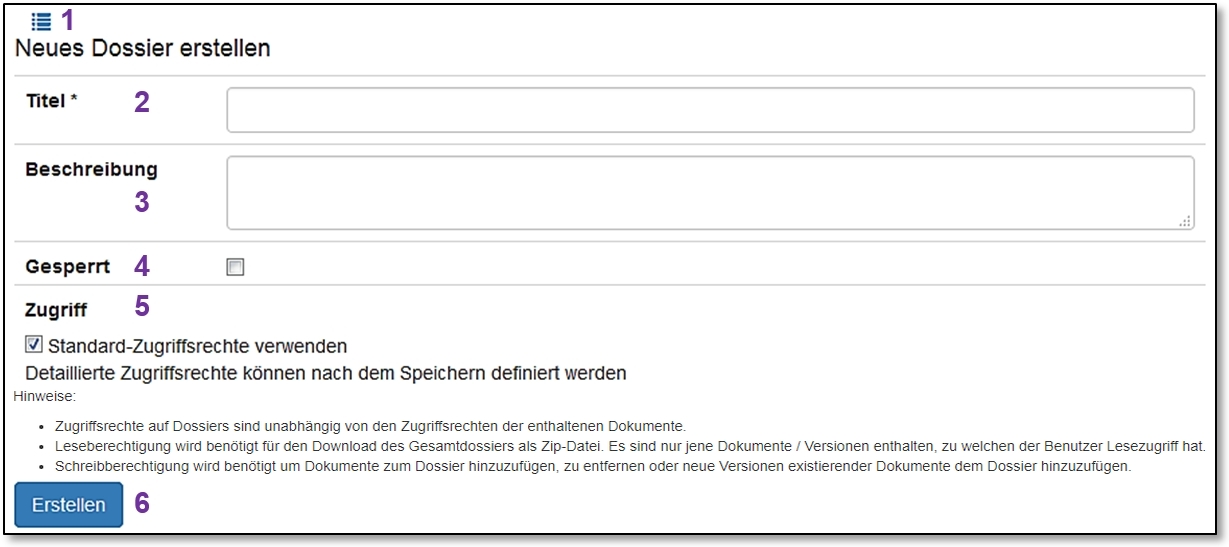
\includegraphics[width=1\linewidth]{../chapters/11_Dokumentenablage/pictures/11-1-1_DossierEingabemaske.jpg}}
\caption{Eingabemaske für neues Dossier}
% \label{fig:speciation}
\end{figure}

Geben Sie einen aussagekräftigen Titel \col{(2)} für ein neues Dossier ein. Sinnvollerweise wird im Titel ein Datumshinweis gemacht, z.B. 'Machbarkeitsstudie XY. August 2015', denn es kann mehrere Dossiers zum selben Thema geben. Es ist auch ratsam vor dem Anlegen eines neuen Dossiers zu prüfen, ob es schon ein Dossier mit einem ähnlichen Titel gibt. In diesem Fall sollte genau der gleiche Text verwendet werden, z.B. 'Machbarkeitsstudie XY. August 2015' und 'Machbarkeitsstudie XY. Dezember 2015'. Bei Bedarf können Sie eine detailliertere Beschreibung \col{(3)} hinterlegen. Dossiers können gegen Veränderungen gesperrt werden. Wird diese Funktion aktiviert, können keine weiteren Dokumente hinzugefügt oder entfernt werden. Setzen Sie dazu das Häkchen bei 'Gesperrt' \col{(4)}. Nun steht das Dossier bei den Dokumenten (im Dropdown-Menü) nicht mehr zur Auswahl zur Verfügung. Dossiers lassen sich bei Bedarf mittels Zugriffsrechte schützen. Wenn keine besonderen Zugriffsrechte erwünscht sind, lassen Sie das Häkchen bei Zugriff \col{(5)} stehen. Soll das Dossier nur für gewisse Nutzergruppen / Personen zugänglich sein, nehmen Sie das Häkchen weg. Später können Sie detailliert bestimmen, wer oder welche Gruppen das Dossier einsehen kann / können. Siehe für die Zugriffsrechte Kapitel \ref{bkm:Ref442273510}. \newline

Wurden sämtliche gewünschten Angaben erfasst, wird das Dossier mit 'Erstellen' \col{(6)} fertiggestellt. Falls Sie zurück zur Übersicht / Liste aller Dossiers gelangen wollen, klicken Sie auf das Listensymbol 
\includegraphics[height=12pt]{/Icons/Listensymbol_zurueck.jpg} \col{(1)}.

\vspace{\baselineskip}

Wurde ein Dossier erfasst und 'Erstellen' geklickt, erscheint folgende Übersicht:

\begin{figure}[H]
\center{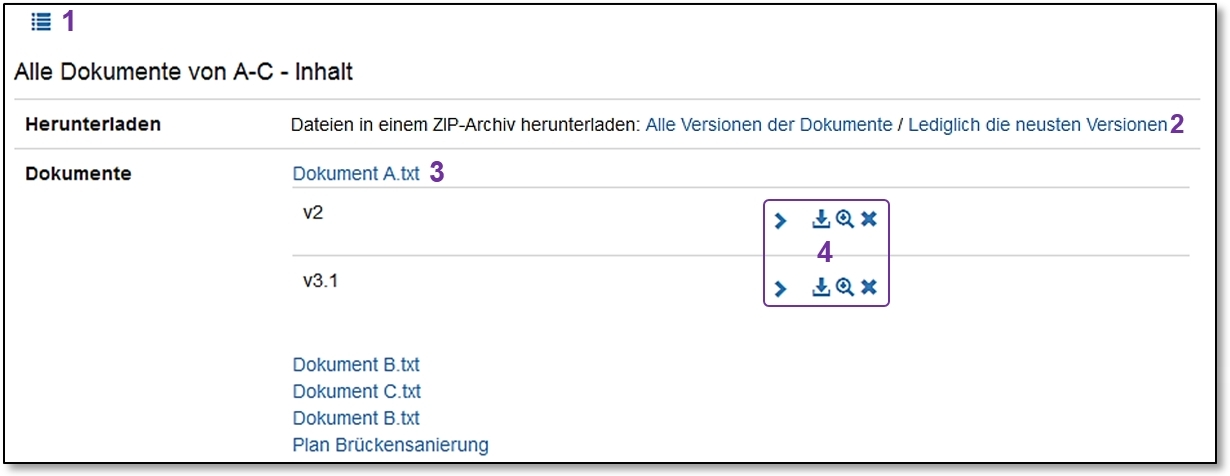
\includegraphics[width=1\linewidth]{../chapters/11_Dokumentenablage/pictures/11-1-1_UebersichtEinesDossiers.jpg}}
\caption{Übersicht des angelegten Dossiers}
% \label{fig:speciation}
\end{figure}

Sie sehen nun Ihren Dossiereintrag. Mit Klick auf das ZIP-Symbol 
\includegraphics[height=12pt]{/Icons/ZIPSymbol.jpg} \col{(2)} können Sie die im Dossier enthaltenen Dokumenten herunterladen. Sie sehen zudem eine Auflistung sämtlicher Dokumente, welche in diesem Dossier enthalten sind. Klicken Sie auf den blauen Dokumententitel \col{(3)} öffnen sich die Optionen (Die Erläuterungen zu den Optionen finden Sie weiter unten). Es ist ersichtlich, welche Haupt- und Unterversionen eines Dokumentes mit dem Dossier verknüpft wurden. Mit erneutem Klick auf den blauen Dokumententitel können Sie die Optionen wieder schliessen.

Mit dem Listensymbol 
\includegraphics[height=12pt]{/Icons/Listensymbol_zurueck.jpg} \col{(1)} gelangen Sie zurück zur Übersicht.

\vspace{\baselineskip}

Das Zuordnen von Dokumenten zu einem Dossier erfolgt im Menüpunkt 'Dokumente' (Menü links 'Dokumentenablage' und dann den Unterpunkt 'Dokumente' auswählen). Um Dokumente zu einem Dossier hinzuzufügen, müssen diese zuerst hochgeladen werden (siehe Kapitel \ref{bkm:Ref442769978}).

\subsubsection{Dossiers betrachten und bearbeiten}

In der Dossiers-Übersicht haben Sie folgende Möglichkeiten:

\begin{figure}[H]
\center{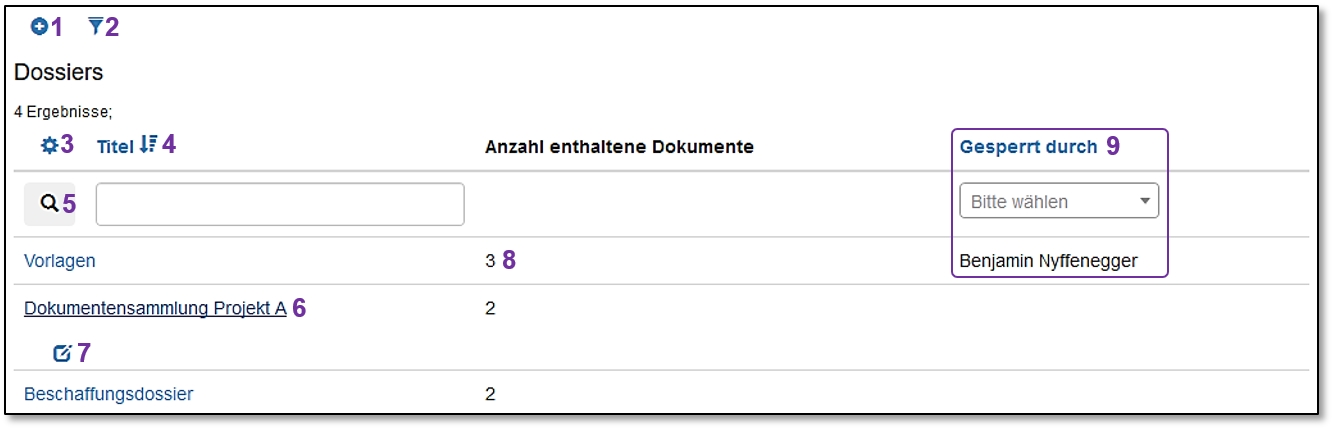
\includegraphics[width=1\linewidth]{../chapters/11_Dokumentenablage/pictures/11-1-2_UebersichtAllerDossiers.jpg}}
\caption{Übersicht aller Dossiers}
% \label{fig:speciation}
\end{figure}

Mit dem Konfigurationssymbol 
\includegraphics[height=12pt]{/Icons/SpaltenEinst.jpg} \col{(1)} lassen sich Spalten beliebig ein- und ausblenden (Da es hier nur eine Spalte gibt, können Sie bei den Dossiers nichts ändern). Mit Klick auf den Text 'Titel' \col{(2)} werden die aufgeführten Dossiers von A-Z, erneut geklickt, von Z-A sortiert.

\vspace{\baselineskip}

\textbf{Suche:} In der Übersicht können Sie nach Dossiers suchen. Ohne einen Platzhalter (*) zu verwenden, können Sie direkt ein Suchwort eingeben und anschliessend auf die Lupe 
\includegraphics[height=12pt]{/Icons/Lupe_kl.jpg} \col{(3)} klicken oder die 'Enter'-Taste drücken. Sämtliche Dossiers, welche das Suchwort beinhalten, werden aufgeführt. \newline

Mit Klick auf den Dossier-Titel \col{(4)} gelangen Sie direkt in die Detail- und Bearbeitungsansicht des Dossiers. Auf der Übersicht sehen Sie zudem auch wie viele Dokumente mit einem Dossier verknüpft sind \col{(5)}. Das Löschen von Dossiers ist momentan nicht möglich. \newline

Haben Sie ein Dossier mittels Klick auf seinen Titel \col{(4)} geöffnet, sehen Sie nebst dem Titel und der Beschreibung auch sämtliche Dokumente, welche das Dossier umfasst:

\begin{figure}[H]
\center{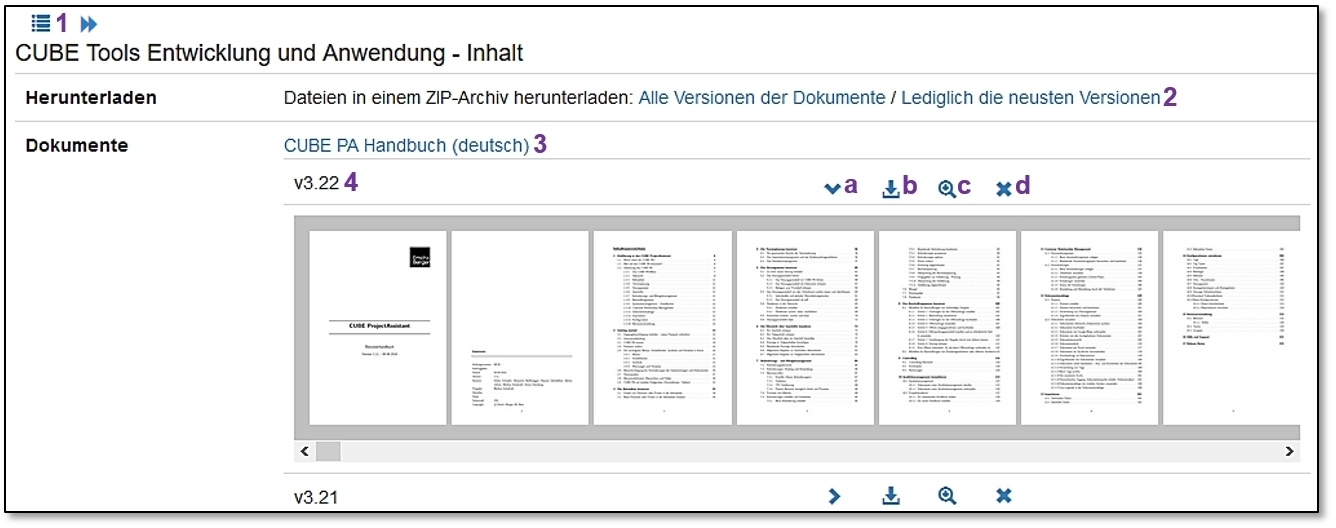
\includegraphics[width=1\linewidth]{../chapters/11_Dokumentenablage/pictures/11-1-2_DetailsEinesDossiers.jpg}}
\caption{Detailansicht des Dossiers}
% \label{fig:speciation}
\end{figure}

Mit dem Listensymbol 
\includegraphics[height=12pt]{/Icons/Listensymbol_zurueck.jpg} \col{(1)} gelangen Sie wieder zur Dossier-Übersicht zurück. Sie können sämtliche im Dossier enthaltenen Dokumente in einem ZIP-Archiv downloaden. Klicken Sie dazu auf das ZIP-Symbol 
\includegraphics[height=12pt]{/Icons/ZIPSymbol.jpg} \col{(2)}. Es öffnet sich ein Dialogfenster (abhängig vom verwendeten Browser) in welchem Sie auswählen können, ob Sie das ZIP-Archiv auf dem Computer speichern oder gerade öffnen wollen. \newline

Weiter sehen Sie die Liste mit sämtlichen Dokumenten, welche in diesem Dossier enthalten sind. Mit Klick auf den blauen Dokumententitel \col{(3)} erscheinen weitere Optionen. Zudem ist ersichtlich, welche Dokumentenversionen bereits mit diesem Dossier verknüpft wurden \col{(4)}. \newline

Es stehen Ihnen nun folgende Optionen zur Verfügung:
Mit dem Kreuzchen-Symbol 
\includegraphics[height=12pt]{/Icons/blKreuzchen.jpg} \col{(d)} können Sie eine bestimmte Version eines verknüpften Dokuments löschen. Bestätigen Sie dazu die Sicherheitsmeldung mit 'OK'.

\begin{figure}[H]
\center{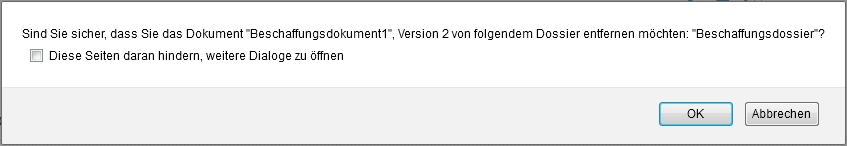
\includegraphics[width=.8\linewidth]{../chapters/11_Dokumentenablage/pictures/11-1-2_DokLoeschen_Meldung.jpg}}
% \caption{Detailansicht des Dossiers}
% \label{fig:speciation}
\end{figure}

Mit dem Lupensymbol 
\includegraphics[height=12pt]{/Icons/Lupe.jpg} \col{(c)} gelangen Sie in den Dokumenteneintrag. Dort können Sie den Dokumenteneintrag ändern, eine neue Dokumentenversion hochladen etc. Näheres zur Dokumentenverwaltung siehe Kapitel \ref{bkm:Ref442273482}. Mit dem Download-Symbol 
\includegraphics[height=12pt]{/Icons/Download.jpg} \col{(b)} ist es möglich eine gewünschte Dokumentenversion herunterzuladen (also nicht das gesamte Dossier). Sie haben je nach Dokumententyp auch die Möglichkeit, das gewünschte Dokument online als Vorschau zu betrachten. Steht diese Option zur Verfügung wird ein rechter Pfeil 
\includegraphics[height=12pt]{/Icons/Pfeil_rechts.jpg} \col{(a)} angezeigt. Klick auf diesen Pfeil öffnet die Vorschau in einem kleinen Fenster (mit erneutem Klick auf den nun erscheinenden Pfeil nach unten können Sie die Vorschau wieder schliessen):

\begin{figure}[H]
\center{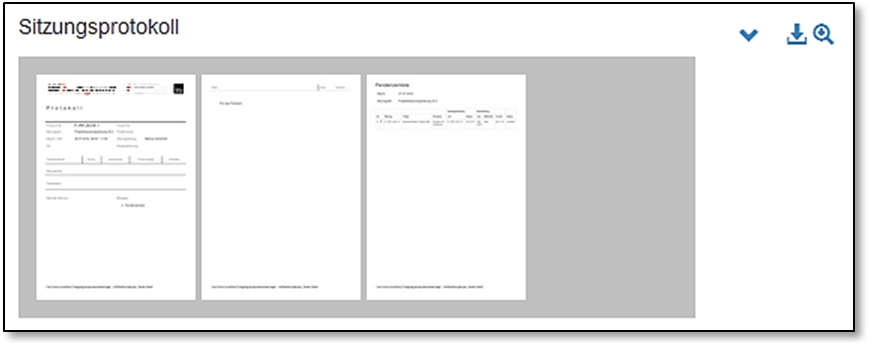
\includegraphics[width=0.75\linewidth]{../chapters/11_Dokumentenablage/pictures/11-1-2_Vorschau.jpg}}
\caption{Die Vorschau im Überblick}
% \label{fig:speciation}
\end{figure}

\pagebreak

Wenn Sie auf eine angezeigte Seite klicken wird die Vorschau im Detail angezeigt:

\vspace{\baselineskip}

\begin{wrapfigure}[12]{r}{9cm}   % [x] Wie manche Zeile soll sich um die Grafik "brechen"
  \vspace{-30pt}      % Grundwert war 20; mit 30 schön oben beim Text ausgerichtet
  \begin{center}
    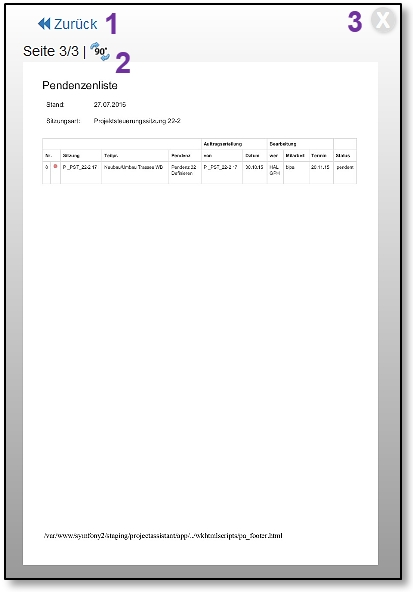
\includegraphics[height=110mm]{../chapters/11_Dokumentenablage/pictures/11-1-2_VorschauDetails.jpg}
  \end{center}
  \vspace{-20pt}
  \caption{Die Vorschau im Detail}
  \vspace{-10pt}
\end{wrapfigure}
Oben links befindet sich die Navigation. Sie sehen wie viele Seite das Dokument umfasst und können mit 'Zurück' und 'Weiter' \col{(1)} durch das Dokument klicken. Wird eine Seite (zum Beispiel eine Karte oder ein Plan) falsch ausgerichtet angezeigt, können Sie mittels dem '90°'-Symbol das Blatt drehen - ein erneuter Klick dreht das Blatt weitere 90° etc. Die Vorschau schliessen sie mit dem 'X' \col{(3)}.

\vspace{5cm}

\subsubsection{Zugriffsrechte bei Dossiers verwalten}
\label{bkm:Ref442273510}
Für jedes Dossier können Sie übergeordnet festlegen wer das Dossier lesen, bearbeiten und/oder löschen darf (Löschen von Dossiers ist in der aktuellen Version noch nicht möglich). Sie können die Zugriffsrechte einer/mehreren Gruppe/n oder einer/mehreren Person/en zuordnen. Das Vorgehen ist in Kapitel \ref{bkm:Ref442869495} beschrieben und erfolgt analog der Zugriffsberechtigung bei Dokumenten.

\pagebreak
\subsection{Dokumente verwalten}
\label{bkm:Ref442273482}

\subsubsection{Dokumenten-Übersicht (Dokumente suchen)}
\label{bkm:Ref443047823}

Wählen Sie im Menü links unter dem Punkt 'Dokumentenablage' den Unterpunkt 'Dokumente' aus. In der Übersicht sehen Sie die erfassten / hochgeladenen Dokumente. Die angezeigten Dokumente werden standardmässig nach der Spalte 'Titel' sortiert. 

\begin{figure}[H]
\center{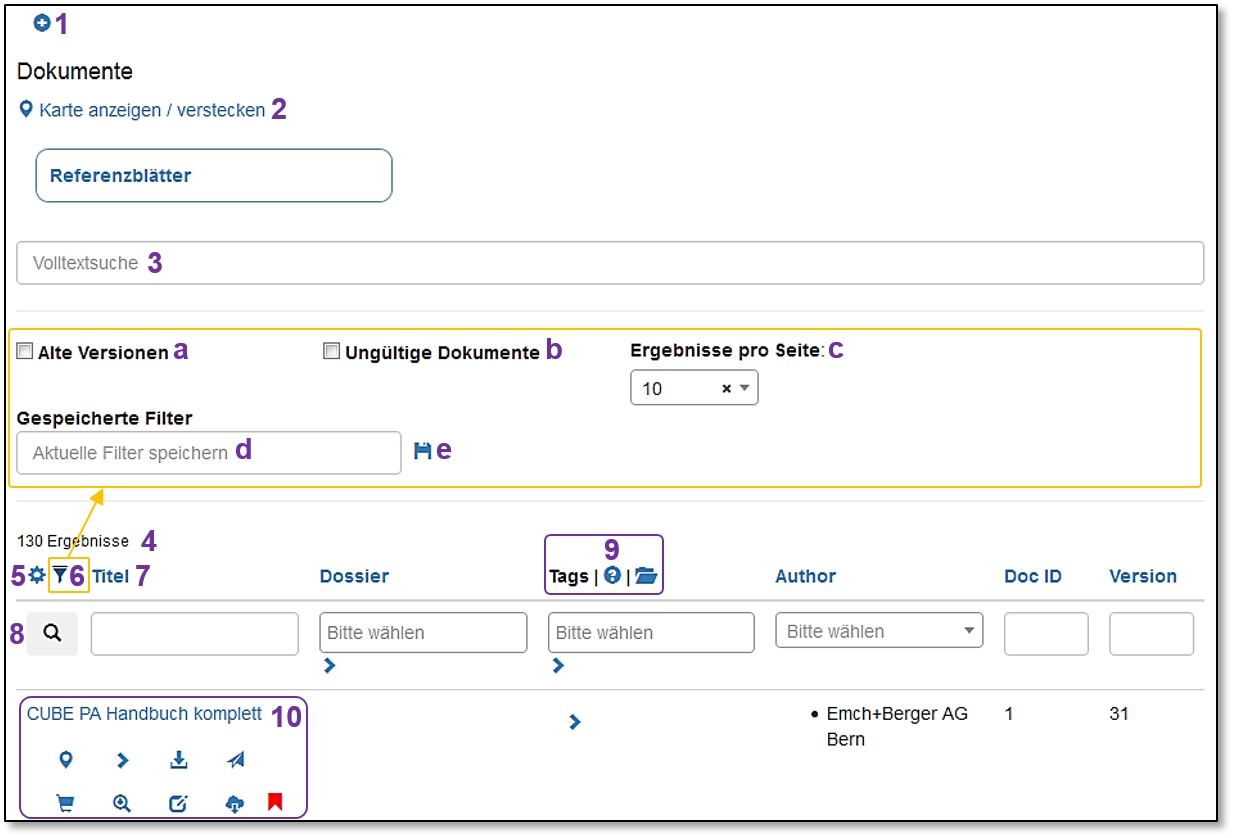
\includegraphics[width=1\linewidth]{../chapters/11_Dokumentenablage/pictures/11-2-1_DokumentenUebersicht.jpg}}
\caption{Übersicht der erfassten Dokumenten}
% \label{fig:speciation}
\end{figure}

Um neue Dokumente hochzuladen, wählen Sie das Plussymbol 
\includegraphics[height=12pt]{/Icons/Plussymbol.jpg} \col{(1)}. Mehr dazu im Kapitel \ref{bkm:Ref442770648}. Mit dem Filtersymbol 
\includegraphics[height=12pt]{/Icons/Filter.jpg} \col{(2)} können Sie die erweiterten Filterfunktionen ein- und ausblenden. Für die Verwendung des erweiterten Filters siehe weiter unten 'Erweiterter Filter' (\ref{bkm:Ref201704051}). Mit dem Nadelsymbol 
\includegraphics[height=12pt]{/Icons/Nadelsymbol.jpg} (Karte anzeigen / verstecken)\col{(3)} können Sie Google-Maps ein- und ausblenden. Auf der Karte werden alle mit Google-Maps verknüpften Dokumente der entsprechenden Suchabfrage angezeigt.\newline

Kundenspezifisch können Tag-Strukturen (Schlagwörter) angelegt werden. Diese ist vergleichbar mit einer Ordnerstruktur im Dateiexplorer. Durch Klick auf einen Ordnerstrukturtitel \col{(4)} kann durch die Struktur navigiert und so nach Tags gesucht werden. Mehr dazu in Kapitel \ref{bkm:Ref201801849} (Hierarchisches Tagging: Dokumentensuche mittels 'Ordnerstruktur'). \newline

Die Volltextsuche \col{(5)} ermöglicht nach beliebigen Begriffen die Einträge zu durchsuchen. Klicken Sie nach Eingabe des Suchwortes auf die Lupe 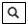
\includegraphics[height=12pt]{/Icons/Lupe_w.jpg} \col{(6)} oder warten Sie bis die Ansicht automatisch gefiltert / aktualisiert wurde. Es können mehrere Suchbegriffe eingegeben werden. Soll eine bestimmte Wortgruppe gesucht werden, sind die Wörter zwischen Anführungszeichen zu setzen. Bei der Volltextsuche werden die Titel von Dokumenten und Dossiers, die Tags sowie wenn technisch möglich der Dokumentinhalt durchsucht. Unterhalb dieser Einstellung sehen Sie jeweils wie viele Datensätze gefunden wurden \col{(7)}.\\
Mit dem Konfigurationssymbol 
\includegraphics[height=12pt]{/Icons/SpaltenEinst.jpg} \col{(8)} können Sie Spalten, welche Sie für die Anzeige nicht benötigen, ausblenden. Nach der Auswahl im erscheinenden Menü klicken Sie dazu auf 'Übernehmen' und schon wird die Ansicht angepasst. \newline

Nebst der Volltextsuche können Sie in den blauen Überschriften \col{(9)} suchen, resp. per Dropdown-Menü auswählen, welche Dokumente angezeigt werden sollen. Mit Klick auf eine blaue Überschrift / einen blauen Spaltentitel wird die angeklickte Spalte von A-Z, mit erneutem Klick, von Z-A sortiert und entsprechend angezeigt. Sie haben die Möglichkeit die hochgeladenen Dokumente mittels 'Tags' zu kennzeichnen. Dazu mehr in Kapitel \ref{bkm:Ref442275849}. \newline
Mit dem Markierungskästchen 
\includegraphics[height=12pt]{/Icons/selectbox.jpg} \col{(10)} können Sie Dokumente markieren (eines oder mehrere) und für sämtlich markierte Dokumente Aktionen wie 'Herunterladen', 'Als E-Mailbeilage versenden' und 'In Papierform versenden' auswählen. Mehr dazu im Kapitel \ref{bkm:Ref201705445} (Dokumentenkorb).

Wenn Sie auf einen aufgelisteten Datensatz klicken \col{(11)} (Unter Titelspalte, blauer Text), öffnen sich die weiteren Optionen. Erneutes Klicken blendet die Optionen wieder aus. Die Optionen werden weiter unten ausgeführt.

\vspace{\baselineskip}

\textbf{Erweiterter Filter:}\\
\label{bkm:Ref201704051}

Mit dem Filtersymbol 
\includegraphics[height=12pt]{/Icons/Filter.jpg} \col{(1)} können die erweiterten Filterfunktionen ein- und ausgeblendet werden:

\begin{figure}[H]
\center{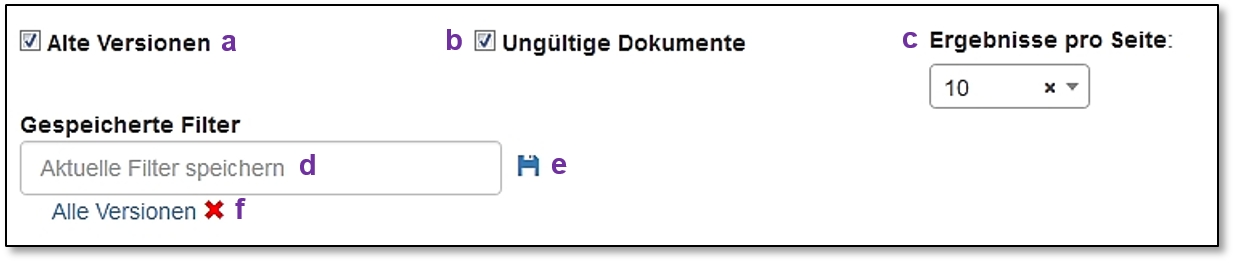
\includegraphics[width=.8\linewidth]{../chapters/11_Dokumentenablage/pictures/11-2-1_FilterEinstellen.jpg}}
\caption{Filtereinstellungen speichern}
% \label{fig:speciation}
\end{figure}

Um ältere Versionen und/oder ungültige Dokumente bei der Suche zu berücksichtigen, setzen Sie bei 'Alte Versionen anzeigen' \col{(a)} und/oder 'Ungültige Dokumente anzeigen' \col{(b)} ein Häkchen. Bei 'Ergebnisse pro Seite' \col{(c)} können Sie die Anzahl Datensätze auswählen, welche auf einer Seite angezeigt werden sollen.\\
Sie können Filtereinstellungen speichern und später wieder aufrufen. Dabei werden die Einstellungen 'Alte Versionen anzeigen' \col{(a)}, 'Ungültige Dokumente anzeigen', die Volltextsuche, Titeleinträge, Doc ID und weitere Spalten berücksichtigt. Die Anzahl angezeigte Datensätze wird in den Filtereinstellungen nicht gespeichert.\\
Haben Sie die gewünschten Einstellungen gemacht, geben Sie einen Filtertitel ein \col{(d)} und klicken auf das Speichernsymbol 
\includegraphics[height=12pt]{/Icons/Diskette.jpg} \col{(e)}. Sämtliche gespeicherten Filtereinstellungen werden nun angezeigt \col{(f)} und können mit Klick auf das rote Kreuzchen 
\includegraphics[height=12pt]{/Icons/roKreuzchen.jpg} \col{(f)} wieder gelöscht werden.


\subsubsection{Dokumente hochladen}
\label{bkm:Ref442863508}\label{bkm:Ref442787515}\label{bkm:Ref442778397}\label{bkm:Ref442770648}\label{bkm:Ref442769978}

\begin{figure}[H]
\center{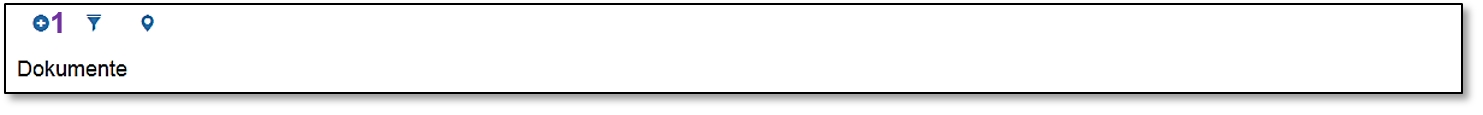
\includegraphics[width=1\linewidth]{../chapters/11_Dokumentenablage/pictures/11-2-2_DokumenteHochladen.jpg}}
% \caption{Neues Dokument hochladen}
% \label{fig:speciation}
\end{figure}

Klicken Sie auf das Plussymbol 
\includegraphics[height=12pt]{/Icons/Plussymbol.jpg} \col{(1)}. Die Eingabemaske für ein neues Dokument erscheint:

\begin{figure}[H]
\center{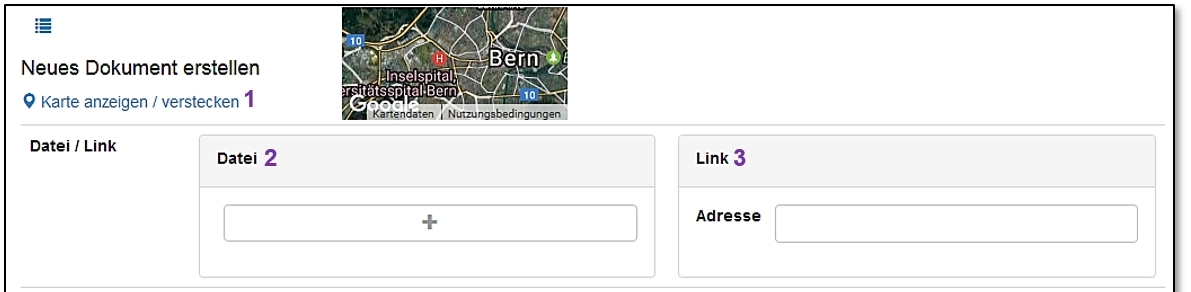
\includegraphics[width=1\linewidth]{../chapters/11_Dokumentenablage/pictures/11-2-2_NeuesDokuErstellen_A.jpg}}
\caption{Eingabemaske für ein neues Dokument}
% \label{fig:speciation}
\end{figure}

Klicken Sie auf den Link 'Karte anzeigen / verstecken' \col{(1)}, um Google-Maps einzublenden, resp. von der kleinen Übersicht auf eine grosse zu wechseln. Wie Sie ein Dokument mit Google-Maps verknüpfen, finden Sie weiter unten im Kapitel \ref{bkm:Ref442545553}. \newline

Sie können nun auswählen, ob Sie eine Datei hochladen \col{(2)} oder einen Internet-Link verknüpfen \col{(3)} wollen.

\vspace{\baselineskip}

\textbf{Eine Datei hochladen:} \col{(2)}
\begin{figure}[H]
\center{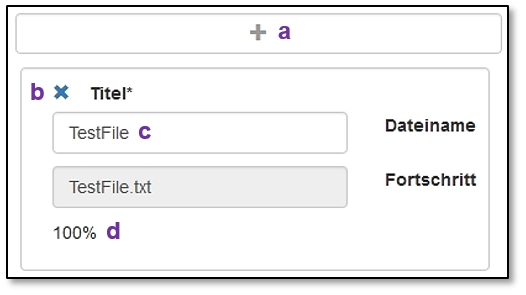
\includegraphics[width=.5\linewidth]{../chapters/11_Dokumentenablage/pictures/11-2-2_Dateititel.jpg}}
\caption{Ein neues Dokument hochladen}
\end{figure}

Klicken Sie auf das graue Plussymbol 
\includegraphics[height=12pt]{/Icons/plus_grau.jpg} \col{(a)} und wählen Sie die gewünschte Datei aus. Alternativ können Sie aus dem Dateiexplorer die gewünschte Datei per 'Drag und Drop' auf das 'Plusfeld' ziehen. Sobald die Datei ausgewählt oder eine Datei in das Feld gezogen wurde, öffnen sich die weiteren Felder \col{(b-d)}. Laden Sie eine grosse Datei hoch, können Sie unter \col{(d)} den Fortschritt des Uploads sehen, resp. ob die Datei vollständig hochgeladen wurde. Der Dateiname \col{(c)} wird übernommen, kann jedoch jederzeit angepasst werden. Der Titel ist ein Pflichtfeld. Haben Sie eine falsche Datei hochgeladen, können Sie mittels dem Kreuzchensymbol 
\includegraphics[height=12pt]{/Icons/Kreuzchen.jpg} \col{(b)} die Datei / den Eintrag wieder löschen. \\
Sie haben auch die Möglichkeit weitere Dateien hochzuladen. Wiederholen Sie die obigen Schritte.

\vspace{\baselineskip}

\textbf{Einen Internet-Link verknüpfen:} \col{(3)}
\begin{figure}[H]
\center{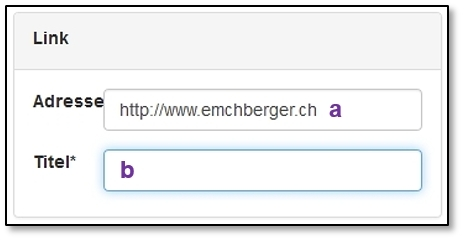
\includegraphics[width=.5\linewidth]{../chapters/11_Dokumentenablage/pictures/11-2-2_Linktitel.jpg}}
\caption{Einen Internet-Link verknüpfen}
\end{figure}

Geben Sie unter 'Adresse' \col{(a)} den gewünschten Internet-Link ein. Ein zusätzliches Feld 'Titel' \col{(b)} erscheint (Pflichtfeld), in welchem Sie einen Titel für den Internet-Link eintragen müssen.\\

Sollten Sie einen fehlerhaften Link eintragen, erscheint folgende Fehlermeldung:

\begin{figure}[H]
\center{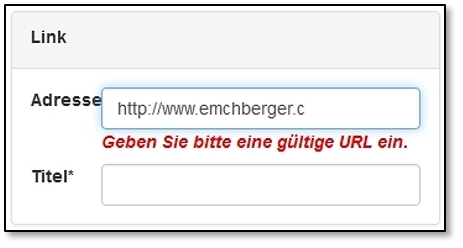
\includegraphics[width=.5\linewidth]{../chapters/11_Dokumentenablage/pictures/11-2-2_Link_Fehler.jpg}}
\caption{Einen Internet-Link verknüpfen}
\end{figure}

\vspace{\baselineskip}

Haben Sie ein Dokument hochgeladen oder einen Internet-Link verknüpft, können Sie nun die weiteren Felder ausfüllen:

\begin{figure}[H]
\center{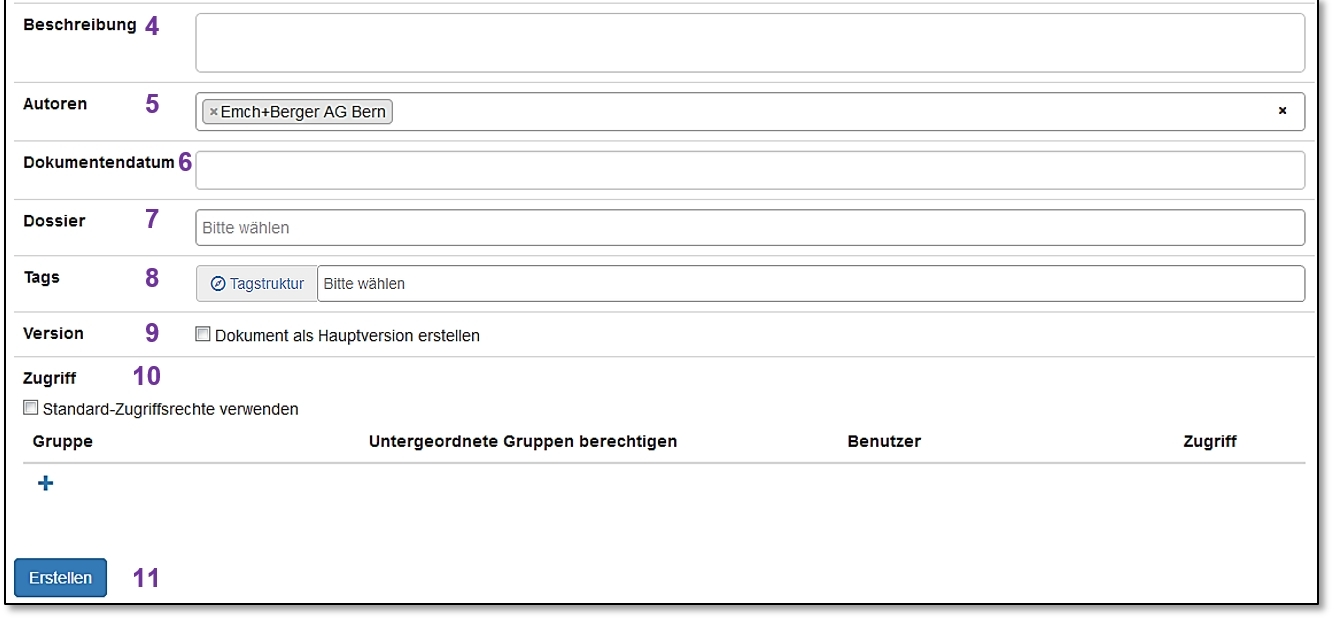
\includegraphics[width=1\linewidth]{../chapters/11_Dokumentenablage/pictures/11-2-2_NeuesDokuErstellen_B.jpg}}
\caption{Eingabemaske für ein neues Dokument}
% \label{fig:speciation}
\end{figure}

\vspace{\baselineskip}

In der Beschreibung \col{(4)} können Sie ergänzende Notizen hinterlegen. Unter Autoren \col{(5)} können Sie mittels Dropdown-Menü die Autoren auswählen. Ein Autor muss vorher erfasst worden sein. Falls ein Autor in der Liste fehlt, kann er durch den Administrator/zentrale Stelle angepasst werden. Geben Sie optional ein Dokumentendatum an \col{(6)}. Soll das Dokument einem Dossier (siehe Kapitel \ref{bkm:Ref442544219}) zugeordnet werden, kann dieses mit dem Dropdown-Menü \col{(7)} ausgewählt werden (Ein Dossier muss zuvor erstellt worden sein). Ein Dokument kann mehreren Dossiers zugeordnet werden. Klicken Sie erneut ins Dropdown-Menü, um das Dokument weiteren Dossiers zuzuordnen. \newline

Dem Dokument können 'Tags' \col{(8)} zugeordnet werden. So ist es später möglich nach bestimmten 'Tags' zu suchen und auf diese Weise Dokumente bestimmter Projekte, Projektphasen, Fachgebiete oder Dokumentenarten zu finden. Tag-Themen (z.B. Fachgebiet) wie auch die einzelnen Tags (z.B. Bahnübergänge, Beleuchtung, Betrieb etc.) können nur durch den Administrator (zentrale Stelle) angepasst resp. ergänzt werden. Fehlt etwas, nehmen Sie bitte mit der entsprechenden Stelle Kontakt auf. Die detaillierte Handhabung mit Tags wird in Kapitel \ref{bkm:Ref201801219} (Verwendung von Tags) beschrieben. \newline

Für jedes hochgeladene Dokument wird ein eigener Eintrag, jedoch mit den gleichen Eingaben der Felder (Beschreibung, Autoren Dossier, etc), erstellt. Gerade für das Zusammenstellen eines Dossiers mit vielen Dokumenten und gleicher Beschreibung, gleichem Autor etc. ist diese Vorgehensweise zeitsparend. 

% Hat ein Dokument seine Gültigkeit verloren, kann dies mit Setzen eines Häkchens \col{(8)} bei den Suchresultaten ausgeschlossen werden. Diese Funktion ist nicht zu verwechseln mit älteren Versionen eines Dokumentes, welche standardmässig bei Suchresultaten nicht angezeigt werden. \newline

Sie können definieren, ob es sich bei einem neu hochgeladenes Dokument um eine Hauptversion (V2, V3. etc.) oder eine Unterversion (V3.1, V3.2 etc.) handelt. Ist das neue Dokument eine Hauptversion setzen Sie das Häkchen bei 'Hauptversion' \col{(9)}. Für ein Dokument können Sie Standard-Zugriffsrechte vergeben \col{(10)} oder gezielt Personen berechtigen. Vergebene Zugriffsrechte können im Bearbeitenmodus später jederzeit wieder angepasst und ergänzt werden. In Kapitel \ref{bkm:Ref442869495} erfahren Sie mehr über die Handhabung der Zugriffsrechte. Damit ein Dokument erstellt werden kann, muss mindestens eine Person berechtigt werden (In der Regel der Erfasser des Dokumentes).

Wurden alle nötigen Eingaben gemacht, wird das Dokument mit 'Erstellen' \col{(11)} hochgeladen und die Einträge gespeichert. \newline

\textbf{Hinweis:} Ein Dokument kann nur durch ein anderes ersetzt werden. Beim Versuch mehrere Dokumente in das Uploadfenster zu ziehen, erscheint folgende Fehlermeldung:

\begin{figure}[H]
\center{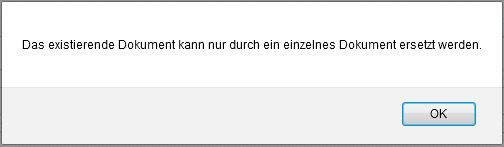
\includegraphics[width=0.75\linewidth]{1122_FehlerDokumentErsetzen.jpg}}
\caption{Fehlermeldung beim Hochladen mehrerer Dateien}
% \label{fig:speciation}
\end{figure}

\textbf{Hinweis:} Wurden bei einem Dokument nur die Metadaten geändert und werden diese gespeichert, wird keine neue Dokumentenversion erstellt. Änderungen der Metadaten werden jedoch in der Änderungshistorie angezeigt. Ebenso, wird die gleiche Datei hochgeladen (in welcher keine Änderungen vorgenommen wurde) oder wird ein Dokument aus- und ohne Änderungen vorzunehmen wieder eingecheckt, erstellt CUBE PA keine neue Dokumentenversion. Es erscheint folgende Meldung:

\begin{figure}[H]
\center{
\includegraphics[width=0.5\linewidth]{../chapters/11_Dokumentenablage/pictures/11-2-2_Meldung_gleicheDatei.jpg}}
\caption{Meldung: Keine neue Dokumentenversion erstellt}
% \label{fig:speciation}
\end{figure}

Um mit der Arbeit weiterfahren zu können, müssen Sie zuerst bei obigem Dialog auf 'OK' klicken.

\subsubsection{Dokumente mit Google-Maps verknüpfen}
\label{bkm:Ref442545553}
Dokumente können mit Google-Maps verknüpft werden. Auf diese Weise ist es möglich, Dokumente eines bestimmten Standortes zu finden, zu bearbeiten oder herunterzuladen. \\
Wechseln Sie mittels dem Bearbeiten-Symbol 
\includegraphics[height=12pt]{/Icons/Bearbeiten.jpg} in den Bearbeitungsmodus des gewünschten Dokumentes (Im Betrachtungsmodus können Sie die Google-Maps-Verknüpfungen anschauen, jedoch keine Verknüpfungen erstellen, hinzufügen oder löschen).

% \vspace{\baselineskip}
\vspace{2mm}

\begin{wrapfigure}[15]{l}{6.5cm}
\vspace{-15pt}
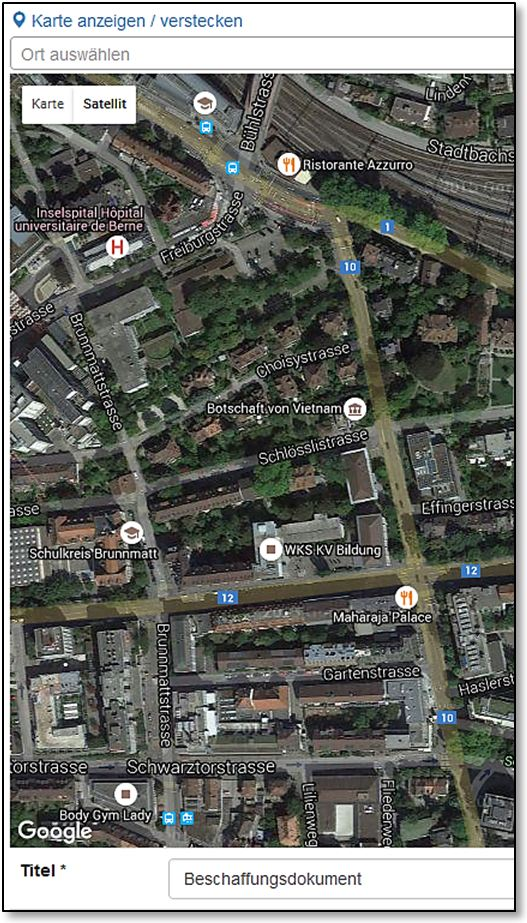
\includegraphics[height=110mm]{1123_GoogleMap.jpg}
% \caption{Status ändern}
\end{wrapfigure}

Um ein Dokument mit einem Ort auf der Karte zu verknüpfen, machen Sie einen Doppelklick mit linker Maustaste auf das Objekt/den gewünschten Ort der Karte. Sie können auch einen vordefinierten Ort auswählen. Klicken Sie dazu in das Eingabefenster 'Ort auswählen' oberhalb der Karte und wählen Sie den gewünschten Ort aus.

\vspace{4mm}

\hspace{15mm} 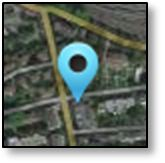
\includegraphics[height=20mm]{1123_GoogleMapNadel.jpg}

Es erscheint obige 'Nadel'. Diese kann per 'Drag \& Drop' später auf eine beliebige Stelle verschoben werden.

\hspace{15mm} 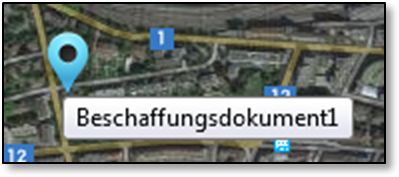
\includegraphics[height=20mm]{1123_GoogleMapText.jpg}

Fahren Sie mit der Maus über die 'Nadel' wird ersichtlich, welches Dokument dahinter verknüpft wurde. \\

Wiederholen Sie obigen Schritt, um weitere Google-Maps-Verknüpfungen hinzuzufügen. Wollen Sie eine bestehende Verknüpfung löschen, klicken Sie mit rechter Maustaste auf die entsprechende Verknüpfung. Es erscheint folgender Dialog, welchen Sie mit 'OK' bestätigen müssen: 

\begin{figure}[H]
\center{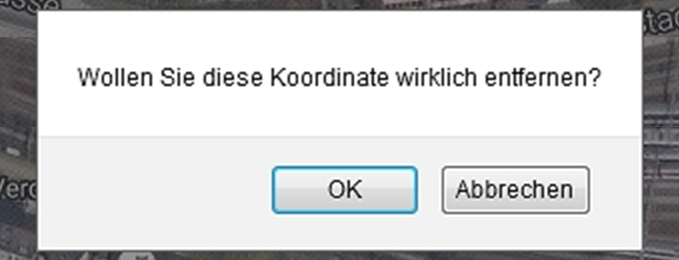
\includegraphics[width=0.5\linewidth]{../chapters/11_Dokumentenablage/pictures/11-2-3_DialogLoeschen.jpg}}
\caption{Verknüpfungen löschen}
% \label{fig:speciation}
\end{figure}

\vspace{\baselineskip}
\pagebreak

\textbf{Handhabung mit Google-Maps im CUBE PA}:

Wenn Sie sich Google-Maps anzeigen lassen, ist die Handhabung wie bei Google-Maps in einem Internet-Browser. Wenn Sie an beliebiger Stelle auf der Karte mit der linken Maustaste klicken und den Klick halten (Maustaste nicht loslassen), können Sie in jede gewünschte Richtung bewegen und so andere Kartenausschnitte erreichen. Wenn Sie bei der Maus ein Scroll-Rad haben und mit dem Mauszeiger über der Karte das Scroll-Rad in die eine Richtung bewegen, wird in den Kartenausschnitt hineingezoomt; das Scroll-Rad in die andere Richtung gedreht, verkleinert sich die Ansicht. (Funktionstasten wie Shift, CTRL, Alt enthalten für die Kartennutzung keine Funktion).

\vspace{\baselineskip}

\textbf{Ein Ort suchen:} 

\begin{figure}[H]
\center{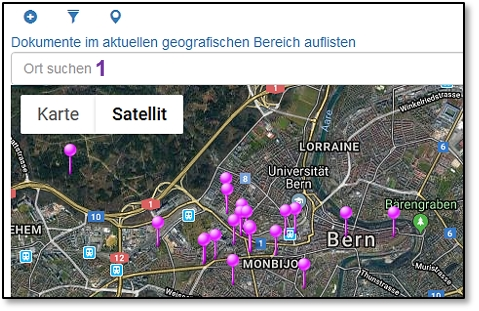
\includegraphics[width=0.6\linewidth]{../chapters/11_Dokumentenablage/pictures/11-2-3_GeographischSuchen.jpg}}
\caption{Ein Ort suchen}
% \label{fig:speciation}
\end{figure}

Wenn Sie sich in der Dokumenten-Übersicht Google-Maps anzeigen lassen (klicken auf 'Karte anzeigen / verstecken'), werden alle mit Google-Maps verknüpften Dokumente auf der Karte angezeigt. Sie können nun einen Ort aus dem Drop-Downmenü auswählen \col{(1)} oder frei nach einem Ort suchen \col{(2)}, indem Sie die Eingaben oberhalb der Karte vornehmen  und anschliessend die 'Enter'-Taste drücken. Durch das übliche Navigieren in Google-Maps gelangen Sie zum gewünschten Kartenausschnitt und sehen sämtliche Dokumente, die darin verknüpft sind. Wenn Sie vorangehend in der Dokumenten-Übersicht eine bestimmte Suchanfrage vorgenommen haben (Filterung), werden in der Karte nur diese Dokumente angezeigt. \newline

\pagebreak
\textbf{Dokumente nach geografischen Bereichen filtern:} \\

\begin{wrapfigure}[9]{r}{7cm}
  \vspace{-35pt}
  \begin{center}
    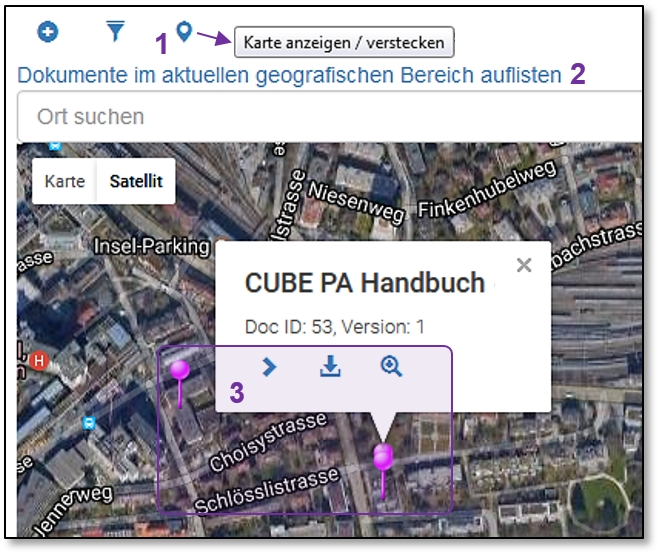
\includegraphics[height=55mm]{../chapters/11_Dokumentenablage/pictures/11-2-3_GeoBereichFilter.jpg}
  \end{center}
  \vspace{-20pt}
  % \caption{Geografische Bereiche filtern}
  \vspace{-10pt}
\end{wrapfigure}
Sie haben die Möglichkeit Dokumente, welche sich auf einen gleichen geographischen Bereich beziehen, resp. mit gleichen / nahen Koordinaten hinterlegt wurden, zu filtern. Sie gehen wie folgt vor: Klicken Sie auf 'Karte anzeigen / verstecken' \col{(1)}, damit die Google-Map angezeigt wird. Nun erscheint oberhalb der Google-Map die Funktion 'Dokumente im aktuellen geografischen Bereich auflisten' \col{(2)}. Klicken Sie diesen Text an. Es wird ein geografischer Filter gesetzt:

\vspace{1cm} 

\begin{wrapfigure}[12]{r}{8cm}
  \vspace{-25pt} 
  \begin{center}
    \includegraphics[height=70mm]{../chapters/11_Dokumentenablage/pictures/11-2-3_GeoBereichResult.jpg}
  \end{center}
  \vspace{-20pt}
  % \caption{Dokumenten in einem gemeinsamen geografischen Bereich}
  \vspace{-10pt}
\end{wrapfigure}
Oberhalb der Suchfelder / Filterfelder erscheint 'Geografischer Filter gesetzt'. Nun werden nur noch diejenigen Dokumente angezeigt, welche mit ähnlichen geografischen Koordinaten verknüpft wurden. In unserem Beispiel sehen Sie nun zwei Dokumente, welche mittels 'Nadel' auch auf vorhergehendem Printscreen angezeigt wurden. \col{(3)}. Es handelt sich dabei um die beiden Dokumente des Suchergebnisses. Wollen Sie den geografischen Filter wieder löschen, klicken Sie dazu auf das kleine Kreuzchen rechts der Meldung 'Geografischer Filter gesetzt' \col{(4)}. Durch erneutes Drücken auf die Lupe \includegraphics[height=12pt]{/Icons/Lupe.jpg} erhalten Sie wieder die ungefilterte Liste.

\subsubsection{Arbeiten mit den hochgeladenen Dokumenten}
\label{bkm:Ref442801819}

\begin{figure}[H]
\center{\includegraphics[width=1\linewidth]{../chapters/11_Dokumentenablage/pictures/11-2-4_FunktionenHochgDateien.jpg}}
\caption{Optionen für hochgeladene Dokumenten}
% \label{fig:speciation}
\end{figure}

In der Dokumenten-Übersicht können Sie nach Dokumenten suchen (siehe Kapitel \ref{bkm:Ref443047823}). Um die verschiedenen Dokumenten-Optionen zu sehen, resp. einzublenden, klicken Sie auf den gewünschten Dokumenten-Titel (blaue Schrift) \col{(1)}. Die Optionen werden eingeblendet. Ein erneuter Klick blendet die Optionen auf dieser Zeile wieder aus. \newline

Sofern das Dokument mit Google-Maps verknüpft ist, gelangen Sie durch Klicken auf das Nadelsymbol \includegraphics[height=12pt]{/Icons/Nadelsymbol.jpg} \col{(2)} direkt zur Karte und auf die verknüpfte Position des Dokuments. Das Symbol wird nur angezeigt, wenn eine Verknüpfung mit Google-Maps vorhanden ist (siehe Kapitel \ref{bkm:Ref442545553}). Folgendes Fenster wird geöffnet:

\begin{figure}[H]
\center{\includegraphics[width=0.5\linewidth]{../chapters/11_Dokumentenablage/pictures/11-2-4_DokAufGoogleMaps.jpg}}
% \caption{Das Menü in CUBE PA}
% \label{fig:speciation}
\end{figure}

Mit dem Kreuzchen rechts oben im Dialogfenster können Sie diese Anzeige schliessen. Sie haben die Möglichkeit von hier aus die Dokumentenvorschau zu öffnen, das Dokument herunterzuladen oder den Dokumenteneintrag anzeigen zu lassen. \newline

Wollen Sie bereits in der Übersicht das Dokument betrachten (Vorschau), können Sie dies mittels dem Pfeilsymbol \includegraphics[height=12pt]{/Icons/Pfeil_rechts.jpg} \col{(3)} tun - insofern die Vorschau das hochgeladene Dateiformat unterstützt. Wollen Sie die Vorschauansicht wieder einklappen, klicken Sie erneut auf das entsprechende Symbol \includegraphics[height=12pt]{/Icons/Pfeil_unten.jpg}. Mehr zur Vorschau weiter unten. \newline

Weiter können Sie das Dokument direkt herunterladen \includegraphics[height=12pt]{/Icons/download.jpg} \col{(4)}, den Dokumenteneintrag mit dem blauen Lupensymbol \includegraphics[height=12pt]{/Icons/Lupe.jpg} \col{(5)} anschauen oder den Dokumenteneintrag mit dem Bearbeiten-Symbol \includegraphics[height=12pt]{/Icons/Bearbeiten.jpg} \col{(6)} bearbeiten. \newline

Wollen Sie ein Dokument online bearbeiten, muss es mittels Symbol \includegraphics[height=12pt]{/Icons/Auschecken.jpg} \col{(7)} ausgecheckt werden. Das Vorgehen ist in Kapitel \ref{bkm:Ref442776572} genauer beschrieben. Durch Klicken auf das graue Favoritensymbol \includegraphics[height=12pt]{/Icons/DokuFlag_grau.jpg} \col{(8)} können Sie ein Dokument zu Ihren persönlichen Favoriten hinzufügen. Das Symbol wird in der Folge rot markiert und das Dokument erscheint in ihrer persönlichen Projektübersicht (siehe Kapitel \ref{bkm:Ref132000001}). Wollen Sie das Dokument nicht mehr als Favorit markiert haben, klicken Sie erneut auf das Favoritensymbol \includegraphics[height=12pt]{/Icons/DokuFlag_rot.jpg}. \newline


\textbf{Umgang mit hinterlegten Links:}

Haben Sie anstelle eines Dokumentes einen Link in CUBE PA hinterlegt, ist die Optionsansicht leicht verändert:

\begin{figure}[H]
\center{\includegraphics[width=1\linewidth]{../chapters/11_Dokumentenablage/pictures/11-2-4_Link_verwenden.jpg}}
\caption{Link öffnen}
% \label{fig:speciation}
\end{figure}

Sie können mittels dem Linksymbol \includegraphics[height=12pt]{/Icons/Link.jpg} \col{(1)} den hinterlegten Link öffnen, wie auch den Link auf Ihrer persönliche Übersicht platzieren, indem Sie auf das Flag-Symbol klicken \includegraphics[height=12pt]{/Icons/DokuFlag_grau.jpg} \col{(2)}. Selbstverständlich können Sie den Link-Eintrag anschauen und bearbeiten. Hingegen fehlen beispielsweise die Optionen 'herunterladen' und 'auschecken'.


\pagebreak
\subsubsection{Dokumentenansicht}
\label{bkm:Ref443047930}

\begin{wrapfigure}[18]{l}{9.5cm}
\vspace{-15pt}
\includegraphics[height=105mm]{../chapters/11_Dokumentenablage/pictures/11-2-5_Dokumentenansicht.jpg}
% \caption{Status ändern}
\end{wrapfigure}

Haben Sie ein Dokument mittels Lupensymbol \includegraphics[height=12pt]{/Icons/Lupe.jpg} geöffnet, sehen Sie nebst dem Titel \col{(1)} sämtliche Informationen (z.B. Autor(en), Tags, die beim Hochladen oder bei späterer Bearbeitung dem Dokument hinzugefügt wurden (siehe Kapitel \ref{bkm:Ref442778397})). Bei fehlenden Angaben bleiben die entsprechenden Felder in der Ansicht leer oder werden nicht angezeigt. Unter dem Titel ist ersichtlich, um welche Dokumentenversion es sich handelt, ebenso welcher Zeitstempel und Bearbeiter hinterlegt sind \col{(2)}. \newline

Unter 'Datei' können Sie mittels \includegraphics[height=12pt]{/Icons/download.jpg} oder Textlink \col{(3)} das aktuelle Dokument herunterladen. Es wird das gewohnte Downloadfenster des Browsers geöffnet, bei welchem Sie auswählen können, ob die Datei geöffnet oder gespeichert werden soll. Mit Klick auf \includegraphics[height=12pt]{/Icons/Versandsymbol.jpg} \col{(4)} können Sie dieses Dokument an beliebige Email-Empfänger versenden. Mehr dazu unter Kapitel \ref{bkm:Ref201701127}. Sie können das Dokument mit Klick auf \includegraphics[height=12pt]{/Icons/shoppingcart_g.jpg} \col{(5)} in den Dokumentenkorb legen. Sobald sich das Dokument im Dokumentenkorb befindet wechselt das Symbol die Farbe: \includegraphics[height=12pt]{/Icons/shoppingcart_r.jpg}. Mit erneutem Klick entfernen Sie das Dokument wieder aus dem Dokumentenkorb. Der Dokumentenkorb wird in Kapitel \ref{bkm:Ref201705445} beschrieben. \newline

Klicken Sie auf das \includegraphics[height=12pt]{/Icons/DokuFlag_grau.jpg} \col{(6)}, um das Dokument in Ihrer persönlichen Übersicht anzeigen zu lassen. Ist das Dokument markiert, wird Ihnen dies mit einem roten Symbol angezeigt: \includegraphics[height=12pt]{/Icons/DokuFlag_rot.jpg}. Mit Klick auf das rote Flag-Symbol wird das Dokument von Ihrer Übersicht wieder entfernt. \newline

Unter 'Statischer Link zu aktuellster Datei-Version' \col{(7)} wird auf die aktuellste Version des Dokuments referenziert. Sie können diesen Link z.B. per Mail versenden und dadurch gewährleisten, dass der Empfänger in jedem Fall auf die aktuellste Version des Dokuments verwiesen wird.

Unter 'Vorschau' \col{(8)} werden die ersten Seiten des Dokuments in einer verkleinerten Darstellung angezeigt.

\vspace{\baselineskip}

Durch Klicken auf eine Seite der Vorschau \col{(9)}, wird das Dokument im Vorschaumodus auf der entsprechenden Seite geöffnet. Der Vorschaumodus wird durch Klicken auf das graue Kreuzchen \includegraphics[height=12pt]{/Icons/X_Button.jpg} \col{(a)} in der rechten oberen Ecke wieder geschlossen. Mit \includegraphics[height=11pt]{/Icons/Weiter.jpg} , respektive \includegraphics[height=11pt]{/Icons/Zurueck.jpg} \col{(b)} können Sie durch die Seiten des Dokuments blättern. Unterhalb der Seitennavigation ist ersichtlich wie viele Seiten das Dokument umfasst \col{(c)}. Mit dem 90°-Symbol \includegraphics[height=12pt]{/Icons/90Grad.jpg} \col{(d)} können Sie die Seiten jeweils um 90° drehen.

\begin{figure}[H]
\center{\includegraphics[width=1\linewidth]{../chapters/11_Dokumentenablage/pictures/11-2-5_Dokumentenvorschau.jpg}}
\caption{Dokumentenvorschau}
% \label{fig:speciation}
\end{figure}

\textbf{Weitere Optionen in der Dokumentenansicht:}

\begin{figure}[H]
\center{\includegraphics[width=1\linewidth]{../chapters/11_Dokumentenablage/pictures/11-2-5_Dokumentenoptionen.jpg}}
\caption{Weitere Optionen für hochgeladene Dokumenten}
% \label{fig:speciation}
\end{figure}

Im Feld 'Datei auschecken' \includegraphics[height=12pt]{/Icons/Auschecken.jpg} \col{(1)} wird die aktuellste Version des Dokuments ausgecheckt (siehe Kapitel \ref{bkm:Ref442780171}). Ist das Dokument einem Dossier zugeordnet, gelangen Sie im Feld 'Dossier' mittels dem blauen Textlink \col{(2)} zum entsprechenden Dossier. Ein Dokument kann mehreren Dossiers zugeordnet werden. \newline

\vspace{\baselineskip}

Unter dem Punkt 'Änderungshistorie' können Sie sich durch Klicken auf das Symbol \includegraphics[height=12pt]{/Icons/Pfeil_rechts_g.jpg} \col{(3)} die Änderungen des Dokuments anzeigen lassen.

\begin{figure}[H]
\center{\includegraphics[width=1\linewidth]{1125_Aenderungshistorie.jpg}}
\caption{Änderungen anzeigen lassen}
% \label{fig:speciation}
\end{figure}

Es wird eine Liste mit den Änderungen ausgeklappt. Ersichtlich sind einerseits vorgenommene Änderungen an den zugehörigen Informationen eines Dokuments (z.B. Autor, Tags) und andererseits Änderungen am Dokument selber (neue Versionen). Klicken Sie auf das Downloadsymbol \includegraphics[height=12pt]{/Icons/Download.jpg} \col{(6)}, um eine alte Version des Dokument herunterzuladen oder auf das Lupensymbol \includegraphics[height=12pt]{/Icons/Lupe.jpg} \col{(5)}, um einen alten Stand des Dokuments anzusehen. \newline

\begin{wrapfigure}[7]{r}{6cm}
\vspace{-25pt}
\includegraphics[height=40mm]{1125_DokumentAeltereVersion.jpg}
% \caption{Status ändern}
\end{wrapfigure}
Wenn Sie eine alte Version eines Dokuments geöffnet haben, erscheint die Warnung \textcolor{red}{'Dies ist nicht die aktuellste Dokumentenversion!'} in der Dokumentenansicht. Wenn Sie jetzt im Feld 'Datei' das Dokument herunterladen, wird nicht auf die aktuellste Version des Dokuments, sondern auf die ausgewählte und angezeigte ältere Version des Dokuments zugegriffen.

\begin{wrapfigure}[7]{r}{6cm}
% \vspace{-15pt}
\includegraphics[height=35mm]{1125_DokumentBearbeiten.jpg}
% \caption{Status ändern}
\end{wrapfigure}
Wollen Sie Angaben zum Dokument bearbeiten oder eine neue Version hochladen, klicken Sie oben links im Fenster auf das Bearbeiten-Symbol \includegraphics[height=12pt]{/Icons/Bearbeiten.jpg} \col{(1)}. Mit dem Listensymbol \includegraphics[height=12pt]{/Icons/Listensymbol_zurueck.jpg} \col{(2)} kehren Sie zur Übersicht zurück. (In der Ansicht einer älteren Version wird das Bearbeiten-Symbol ausgeblendet. Sie können lediglich mit dem Listensymbol \includegraphics[height=12pt]{/Icons/Listensymbol_zurueck.jpg} zur Übersicht zurückkehren.)

\vspace{\baselineskip}

\textbf{Details zur Änderungshistorie} \\
In der Änderungshistorie werden sämtliche Änderungen festgehalten. Einerseits wird dokumentiert, wenn eine neues Dokument (eine überarbeitete Version) hochgeladen wird, andererseits werden beispielsweise Änderungen an den Metadaten ebenfalls in der Änderungshistorie festgehalten, ohne jedoch eine neue Dokumentenversion zu erzeugen (siehe Kapitel \ref{bkm:Ref442863508}).

\begin{figure}[H]
\center{\includegraphics[width=1\linewidth]{../chapters/11_Dokumentenablage/pictures/11-2-5_AenderungshistorieUebersicht.jpg}}
\caption{Die Änderungshistorie in der Übersicht}
% \label{fig:speciation}
\end{figure}

\col{(1)} In der Änderungshistorie wird jeweils diejenige Version mit 'fetter' Schrift angezeigt, welche gerade im Ansichtsmodus geöffnet ist. Sie sehen ebenfalls, um welche Version es sich handelt. Die verschiedenen Einträge werden mit einem Strich abgetrennt \col{(2)}. Alle Änderungen werden festgehalten: Erster Eintrag: Eine neue Datei wurde hochgeladen und eine Beschreibung (Metadaten) hinzugefügt. Im zweiten Eintrag wurde das Dokument lediglich dem Beschaffungsdossier hinzugefügt. Sie sehen wann dies von wem gemacht wurde. Wenn Sie die Vorschau der aktuellen oder einer früheren Version öffnen möchten, klicken Sie auf das Pfeilsymbol \includegraphics[height=12pt]{/Icons/Pfeil_rechts.jpg} \col{(3)}. Es öffnet sich die Vorschau. Klicken Sie auf eine der Vorschauseiten, wird diese gross angezeigt und Sie haben die Möglichkeit durch das Dokument zu navigieren oder eine Seite um jeweils 90° zu drehen. Mit dem Kreuzchen oben rechts \includegraphics[height=12pt]{/Icons/X_Button.jpg} schlissen Sie die grosse Vorschau, mit Klick auf das Pfeilsymbol (Pfeil nach unten \includegraphics[height=12pt]{/Icons/Pfeil_unten.jpg}) klappen Sie die kleine Vorschau wieder zu.

Sie können in der Änderungshistorie die aktuelle oder eine frühere Dokumentenversion mittels dem Download-Symbol \includegraphics[height=12pt]{/Icons/download.jpg} \col{(4)} direkt herunterladen. Mit dem Lupensymbol \includegraphics[height=12pt]{/Icons/Lupe.jpg} \col{(5)} gelangen Sie in die Übersicht der entsprechenden (frühere) Version. Ebenfalls haben Sie die Möglichkeit Metadaten einer früheren Version zu verändern. Dazu klicken Sie auf das Bearbeitungssymbol \includegraphics[height=12pt]{/Icons/Bearbeiten.jpg} \col{(6)}. Vergewissern Sie sich jeweils vor einem Bearbeiten, dass Sie sich in der gewünschten Dokumentenversion befinden.

\vspace{\baselineskip}

\textbf{Hinweis:} Das Ändern von älteren Dokumentenversionen (Metadaten, Zugriffsrechte) ist nur wie oben beschrieben über die Änderungshistorie möglich.

\pagebreak

\textbf{Neue Version eines Dokuments hochladen}

\vspace{\baselineskip}

\begin{wrapfigure}[13]{r}{6cm}
\vspace{-35pt}
\includegraphics[height=100mm]{1125_DokumentBearbeitenFelder.jpg}
% \caption{Status ändern}
\end{wrapfigure}
Im Bearbeitungsmodus können Sie die Angaben zum Dokument ergänzen (siehe dazu die Ausführungen im Kapitel \ref{bkm:Ref442787515}). Wenn Sie eine neue Version eines Dokuments hochladen wollen, klicken Sie unter Datei auf 'Durchsuchen' \col{(1)} und wählen die gewünschte Datei aus. Bei Bedarf können die weiteren Einträge (Metadaten) angepasst werden.

\vspace{\baselineskip}

Wurden alle nötigen Eingaben gemacht, wird das Dokument mit \includegraphics[height=12pt]{/Icons/B_Uebernehmen.jpg} unten links hochgeladen und die Einträge gespeichert. Der alte Stand (Dokument und Metadaten) bleiben gespeichert und können in der 'Änderungshistorie' der Dokumentenansicht jederzeit wieder aufgerufen werden.

\vspace{\baselineskip}
\vspace{\baselineskip}

\textbf{Hinweis}: Sind mehrere Versionen eines Dokuments dem gleichen Dossier zugeordnet, wird automatisch nur die aktuellste Version dem Dossier angehängt. Dies gilt es besonders beim Hochladen von neuen Versionen von Dokumenten zu beachten. Soll beispielsweise eine neue Version eines Dokuments nicht mehr einem bestimmten Dossier zugeordnet werden, ist gleichzeitig mit dem Hochladen des Dokuments im Feld 'Dossier' der Eintrag zu löschen (aufs 'x' klicken bei der Zeile Dossier) \col{(2)}. Dadurch wird die alte Version des Dokuments im Dossier nicht 'überschrieben'.

\begin{figure}[H]
\center{\includegraphics[width=1\linewidth]{1125_DokEintragLoeschen.jpg}}
\caption{Eintrag löschen}
% \label{fig:speciation}
\end{figure}


\subsubsection{Dokumentenkorb}
\label{bkm:Ref201705445}
% Neues Kapitel

Der Dokumentenkorb hat eine ähnliche Funktion wie der bekannte Warenkorb eines Online-Shops. Über den Dokumentenkorb können verschiedene Funktionen wie der kombinierte Download als Zip-Archiv, Direktversand per Mail sowie Planrepro bedient werden. So ist es möglich, eine beliebige Anzahl Dokumente in den Dokumentenkorb zu legen und anschliessend die gewünschte Funktion für sämtliche Dokumente im Korb auszuführen.

\vspace{\baselineskip}

Gehen Sie wie folgt vor:

\begin{figure}[H]
\center{\includegraphics[width=1\linewidth]{../chapters/11_Dokumentenablage/pictures/11-dkorb_Dokumentenkorb_Uebersicht1.jpg}}
\caption{Der Dokumentenkorb verwenden}
% \label{fig:speciation}
\end{figure}

Suchen Sie mittels Volltextsuche, dem Filter oder der Navigation durch die Dokumente das gewünschte Dokument, welches in den Dokumentenkorb gelegt werden soll. Markieren Sie das Dokument mit Klick auf das Kästchen \col{(1)}. Wiederholen Sie diesen Schritt bis Sie sämtliche Dokumente ausgewählt haben, die Sie weiterverarbeiten wollen. Oben in der Liste erscheinen nun die möglichen Optionen \col{(2)}. Sie haben auch weiterhin die Möglichkeit, die bekannten Optionen unterhalb des Titels zu nutzen \col{(8)}. \\
Nun haben Sie folgenden Möglichkeiten: Mit Klick auf den Dokumentenkorb \includegraphics[height=12pt]{/Icons/dk_korb_b.jpg} \col{(3)} können Sie auswählen, ob sämtliche sich im Dokumentenkorb befindlichen Dokumente gelöscht werden sollen \col{(a)} oder ob Sie die ausgewählten Dokumente aufgelistet haben wollen \col{(b)}:
\begin{figure}[H]
\center{\includegraphics[width=.25\linewidth]{../chapters/11_Dokumentenablage/pictures/11-dkorb_Auswahl.jpg}}
% \caption{Weitere Optionen}
% \label{fig:speciation}
\end{figure}

Mit Klick auf das Flagsymbol \includegraphics[height=12pt]{/Icons/dk_flag_b.jpg} \col{(4)} werden sämtlich ausgewählte Dokumente in ihrer persönlichen Übersicht als Favoriten angezeigt. \\
Mit Klick auf das Downloadsymbol \includegraphics[height=12pt]{/Icons/dk_download.jpg} \col{(5)} werden sämtliche sich im Dokumentenkorb befindlichen Dokumente per ZIP-File heruntergeladen. Wollen Sie die angewählten Dokumente per Mail versenden, klicken Sie auf das Versandsymbol \includegraphics[height=12pt]{/Icons/dk_senden.jpg} \col{(6)}. Mehr dazu im Kapitel \ref{bkm:Ref201701127} (Dokumente per Email versenden). Sie haben auch die Möglichkeit, die ausgewählten Dokumente per Papierform zu versenden. Dazu klicken Sie auf das Drucker-Symbol \includegraphics[height=12pt]{/Icons/dk_drucken.jpg} \col{(7)}. Wie Sie diese Funktion im Detail nutzen finden Sie im Kapitel \ref{bkm:Ref20170609127} (Druckaufträge an Reprozentren).

\vspace{\baselineskip}

Wird nur ein Dokument in den Dokumentenkorb gelegt, werden Ihnen oben in der Liste mehrere Optionen angeboten:

\begin{figure}[H]
\center{\includegraphics[width=.8\linewidth]{../chapters/11_Dokumentenablage/pictures/11-dkorb_weitereOptionen.jpg}}
\caption{Weitere Optionen}
% \label{fig:speciation}
\end{figure}

Zu den oben beschrieben Optionen können zusätzlich mit Klick auf die Lupe \includegraphics[height=12pt]{/Icons/dk_lupe.jpg} \col{(1)} die Details des ausgewählte Dokuments betrachten, den Eintrag bearbeiten \includegraphics[height=12pt]{/Icons/dk_bearb.jpg} \col{(2)}, einen geographischen Punkt auf Google-Map setzen \includegraphics[height=12pt]{/Icons/dk_nadel.jpg} \col{(3)} oder das Dokument auschecken \includegraphics[height=12pt]{/Icons/dk_auschecken.jpg} \col{(4)}. Diese Knöpfe entsprechen den gleichen Optionen wie die Icons unterhalb eines Dokumenten-Titels.

\vspace{\baselineskip}

\textbf{Hinweis:} Wird mittels Klick auf das Warenkorb-Symbol die Auswahl der markierten Dokumenten angezeigt, wird die Farbe des Symbols rot dargestellt \includegraphics[height=12pt]{/Icons/dk_korb_r.jpg}. Ebenso, wurde für die ausgewählten Dokumente das Favoriten-Symbol angeklickt, ändert sich wie gewohnt die Farbe \includegraphics[height=12pt]{/Icons/dk_flag_r.jpg} \col{(1)}:

\begin{figure}[H]
\center{\includegraphics[width=.75\linewidth]{../chapters/11_Dokumentenablage/pictures/11-dkorb_Dokumentenkorb_Uebersicht2.jpg}}
\caption{Angezeigter Warenkorb / Auswahlanzeige beenden}
% \label{fig:speciation}
\end{figure}

\textbf{Hinweis:} Mit Klick auf das runde Kreuzchen-Symbol \includegraphics[height=12pt]{/Icons/FilterLoeschen_b.jpg} \col{(2)} können Sie den Auswahlanzeigemodus beenden. 

\vspace{\baselineskip}

\textbf{Beschreibung der einzelnen Optionen:}

\subsubsection{Dokumente per Email versenden}
\label{bkm:Ref201701127}
% Neues Kapitel

Es ist möglich, Dokumente direkt aus der Dokumentenablage per Mail an beliebige Empfänger zu versenden. Der Versand von Dokumenten wird zu Gunsten der Nachvollziehbarkeit und Transparenz in der Änderungshistorie aufgezeichnet.

Klicken Sie auf das Versandsymbol \includegraphics[height=12pt]{/Icons/Versandsymbol.jpg}, um sämtliche Dokumente im Dokumentenkorb an eine oder mehrere Emailadressen zu versenden. Sie können vor dem Absenden immer noch Dokumente löschen, welche Sie nicht versenden wollen.

\begin{figure}[H]
\center{\includegraphics[width=1\linewidth]{../chapters/11_Dokumentenablage/pictures/11-dkorb_Dok_versenden}}
\caption{Dokumente versenden}
% \label{fig:speciation}
\end{figure}

Empfänger eintragen \col{(1)}: Geben Sie bei 'Empfänger' eine oder mehrere Emailadressen ein. Trennen Sie die Emailadresse mittels ';' oder einem Leerschlag.
Unter 'Nachricht' \col{(2)} können Sie für den oder die Empfänger die nötigen Informationen eingeben. Sie sehen sämtliche ausgewählten Dokumente, welche an den oder die Empfänger versendet werden und können beliebige Dokumente mittels dem Kreuzchen \includegraphics[height=12pt]{/Icons/blKreuzchen.jpg} \col{(3)} auch wieder löschen. Die Grösse sämtlicher Dokumenten ist unter \col{(4)} ersichtlich. Haben Sie alle nötigen Angaben und Texte gemacht, klicken Sie auf 'Senden' \col{(5)}, um den Sendeauftrag abzuschliessen.

\vspace{\baselineskip}

Nun erscheint eine Bestätigungsmeldung, an welche Empfänger das Email mit den Dokumenten versendet worden ist:

\begin{figure}[H]
\center{\includegraphics[width=.4\linewidth]{../chapters/11_Dokumentenablage/pictures/11-dkorb_Sendebestaetigung}}
\caption{Versand-Bestätigung}
% \label{fig:speciation}
\end{figure}

Per Email wird Ihnen nochmals mitgeteilt, welche Dokumente an welche Empfänger versendet wurden. Falls Emails einen Empfänger nicht erreicht haben, wird dies ebenfalls aufgeführt.

\vspace{\baselineskip}

\subsubsection{Dokumente als Zip-Archiv herunterladen}
% Neues Kapitel

Sie haben die Möglichkeit, sämtliche im Dokumentenkorb liegenden Dateien in einem Zip-Archiv herunterzuladen. Klicken Sie dazu auf das Download-Symbol in der Dokumentenkorbliste, um sämtliche im Dokumentenkorb abgelegten Dokumente als Zip-Archiv herunterzuladen.

\vspace{\baselineskip}

Es öffnet sich das Downloadfenster Ihres Browsers. Wählen Sie 'Öffnen' oder 'Datei speichern', um das Zip-Archiv im Datei-Explorer zu öffnen, resp. auf Ihrem Computer abzuspeichern:

\begin{figure}[H]
\center{\includegraphics[width=.5\linewidth]{../chapters/11_Dokumentenablage/pictures/11-dkorb_DokDownload}}
\caption{Dokumente als Zip-Archiv herunterladen}
% \label{fig:speciation}
\end{figure}

\subsubsection{Druckaufträge an Reprozentren}
\label{bkm:Ref20170609127}
% Neues Kapitel

Pläne können direkt aus der Dokumentenablage an Reprozentren zur Direktauslieferung von geplotteten Plänen gesendet werden. Mehrere Pläne können im Rahmen einer einzigen Bestellung an mehrere Empfänger verschickt werden, wobei die Ausführung (Anzahl Exemplare, Druck-/elektronische Kopie) pro Empfänger separat festgelegt werden kann.

\vspace{\baselineskip}

Für das Versenden von Plänen via Reprozentren gehen Sie wie folgt vor: Wählen Sie wie oben beschrieben sämtliche benötigten Dokumente / Pläne aus und legen Sie diese in den Dokumentenkorb. In Ihrem Dokumentenkorb sehen Sie nun alle ausgewählten Dokumente. Haben Sie zu viele Dokumente ausgewählt / markiert, können Sie bei diesen Dokumenten die Markierung wieder herausnehmen \includegraphics[height=12pt]{/Icons/checkbox_markiert.jpg} $ > $ \includegraphics[height=12pt]{/Icons/checkbox_leer.jpg} und den Warenkorb entsprechend anpassen. Sind alle Dokumente / Pläne beisammen, klicken Sie im Dokumentenkorb auf das Drucker-Symbol \includegraphics[height=12pt]{/Icons/printer.jpg}. Es öffnet sich folgendes Fenster:

\begin{figure}[H]
\center{\includegraphics[width=1\linewidth]{../chapters/11_Dokumentenablage/pictures/11-dkorb_ReproDialog1.jpg}}
\caption{Dialogfenster 'Allgemeine Angaben' für die Planlieferung}
% \label{fig:speciation}
\end{figure}

Wählen oder ergänzen Sie folgende Felder:

\textbf{Projekt:} Dies ist ein Pflichtfeld. Wählen Sie in der vordefinierten Liste der eingetragenen Projekt das entsprechende Projekt aus. \\
\textbf{Teilprojekt / Objekt:} Mittels Freitext können Sie hier ergänzende Informationen zum Projekt hinterlegen. \\
\textbf{Reprozentrum:} Dies ist ein Pflichtfeld. Sämtliche in den Voreinstellungen (Konfiguration) hinterlegten Reprozentren können Sie hier für die Planlieferung auswählen. \\
\textbf{Priorität:} Dies ist ein Pflichtfeld. Sie können zwischen drei verschiedenen Prioritäten auswählen:
\begin{figure}[H]
\center{\includegraphics[width=1\linewidth]{../chapters/11_Dokumentenablage/pictures/11-dkorb_ReproPrio}}
\caption{Prioritätenauswahl für Planlieferung}
% \label{fig:speciation}
\end{figure}
Beachten Sie, dass die Auslieferung auch abhängig ist von der Bestellzeit. Für Detailklärung kontaktieren Sie die zuständigen Stellen. \\
\textbf{Auslieferungsdatum:} Dies ist ein Pflichtfeld. Das Auslieferungsdatum wird automatisch in Abhängigkeit der gewählten Priorität gesetzt und kann nachträglich geändert werden. \\
\textbf{Zweck:} Sie können hier aus einer Liste vordefinierter Angaben einen oder mehrere Zweck(e) auswählen, welche/r dann auf dem Lieferschein für die Empfänger erscheint.
\begin{figure}[H]
\center{\includegraphics[width=1\linewidth]{../chapters/11_Dokumentenablage/pictures/11-dkorb_ReproZweck}}
\caption{Zweckangabe für den Lieferschein}
% \label{fig:speciation}
\end{figure}
\textbf{Mitteilung an Empfänger:} Hier können Sie mittels Freitext die nötigen Angaben für den/die Empfänger eingeben. \\
\textbf{Mitteilung ans Reprozentrum:} Diese Angaben sind nach Abschluss der Planbestellung für das Reprozentrum sichtbar. \\
\textbf{Beilagen:} Pro Dokument, welches im Dokumentenkorb war und nun für die Planlieferung zur Verfügung steht, können Sie Detailangaben vornehmen.   Mit Klick auf den blauen Dokumententitel können Sie das Dokument / den Plan nochmals öffnen oder auf Ihrem Computer abspeichern.
In der Regel wird die Grösse des Plans in Abhängigkeit des PDF's bestimmt. Sie haben jedoch die Möglichkeit hier Einfluss zu nehmen und Anpassungen des Format dem Reprozentrum mitzuteilen. Zudem können Sie pro Dokument / Plan auswählen, ob dieser in Farbe oder s/w ausgedruckt und geliefert werden soll. Sie können abschliessend noch definieren, in welcher Form / Endbearbeitung der Plan auf die Baustelle oder in ein Büro geliefert werden soll (Falten, Heften, Heftstreifen, Nach Absprache, Rollen, Spiralbinden, Thermobindung).
Haben Sie alle nötigen Angaben gemacht, klicken Sie auf 'Weiter zu Seite 2' um zu den 'Empfängerdetails' zu gelangen:

\begin{figure}[H]
\center{\includegraphics[width=1\linewidth]{../chapters/11_Dokumentenablage/pictures/11-dkorb_ReproDialog2.jpg}}
\caption{Dialogfenster 'Empfängerdetails' für die Planlieferung}
% \label{fig:speciation}
\end{figure}

Hier können Sie einen oder mehrere Empfänger auswählen. Gehen Sie wie folgt vor: aus der Dropdownliste 'Empfänger hinzufügen' wählen Sie die gewünschte Person aus. Wiederholen Sie diesen Schritt mit weiteren benötigten Empfängern. So bald Sie einen Empfänger aus der Liste ausgewählt haben, erscheint dieser unten im Dialogfenster. Sie können nun noch einige Einstellungen vornehmen, wie zum Beispiel wie viele Exemplare pro Empfänger benötigt werden und ob der / die Empfänger die Pläne ausgedruckt (Druckexemplar) oder als PDF/Dokument per E-Mail zugestellt benötigt / benötigen (elektronisch). \\
Sie haben nun die Möglichkeit individuelle Nachrichten an die einzelnen Empfänger zu versenden (E-Mail / Lieferschein) \col{(2)}. Werden hier nun Nachrichten hinterlegt, werden die allgemeinen Nachrichten auf der ersten Dialogseite (Allgemeine Angaben) dadurch ersetzt (Siehe auch Information mit Klick auf \includegraphics[height=12pt]{/Icons/Info_blau.jpg}. \col{(2)}\\
Mit dem Mülltonnensymbol \includegraphics[height=12pt]{/Icons/Muelltonne.jpg} \col{(3)} können Sie die ausgewählten Empfänger wieder löschen. Werden mittels obiger Dropdownliste 'Empfänger hinzufügen' \col{(1)} Empfänger ausgewählt, welche bereits unten in der Liste stehen, erscheint folgende Meldung:

\begin{figure}[H]
\center{\includegraphics[width=.5\linewidth]{../chapters/11_Dokumentenablage/pictures/11-dkorb_Meldung_doppeltePerson.jpg}}
\caption{Meldung: Empfänger existiert bereits}
% \label{fig:speciation}
\end{figure}

\vspace{\baselineskip}

Müssen Sie nochmals bei den 'Allgemeinen Angaben' Änderungen vornehmen oder diese kontrollieren, können Sie mittels Klick auf 'Weiter zu Seite 1' wieder zu diesen Angaben gelangen. Ist alles in Ordnung und wollen Sie die Pläne wie nun definiert bestellen, klicken Sie auf 'Auftrag absenden'. In der Folge öffnet sich der Lieferschein und die entsprechenden Emails werden verschickt. Das Reprozentrum erhält den Auftrag per Email mit einem Link in den CUBE PA. Dort können sie den Auftrag bearbeiten. Wurde der Auftrag durch das Reprozentrum bearbeitet, resp. ausgelöst, wird durch das Reprozentrum die Bestellung als 'abgeschlossen' markiert. Dies wird dem Besteller so auch protokolliert.

\vspace{\baselineskip}

Wurde eine Bestellung ausgelöst, wird diese beim Besteller (Bearbeiter des CUBE PA) in der Übersicht angezeigt. Wurde durch das Reprozentrum wie oben beschrieben der Auftrag / die Bestellung als 'abgeschlossen' markiert, wird dies ebenfalls in der Übersicht angezeigt.

\vspace{\baselineskip}

\textbf{Wichtiger Hinweis:} Wird während den Eingaben in oben beschrieben Formularen auf das Kreuzchen \includegraphics[height=12pt]{/Icons/X_BUtton.jpg} (rechts oben) geklickt, verlieren Sie sämtliche Einstellungen/Eingaben. Die Dokumente / Pläne bleiben noch im Dokumentenkorb und Sie können wieder mit einem neuen Auftrag beginnen.

\subsubsection{Zugriffsrechte bei Dokumenten verwalten}
\label{bkm:Ref442869495}

Für jedes Dokument können Sie festlegen wer das Dokument lesen, bearbeiten und/oder löschen darf (Löschen von Dokumenten ist in der aktuellen Version nicht möglich). Sie können die Zugriffsrechte einer/mehreren Gruppe/n oder einer/mehreren Person/en zuordnen:

\begin{figure}[H]
\center{\includegraphics[width=1\linewidth]{../chapters/11_Dokumentenablage/pictures/11-berecht_Rechte.jpg}}
\caption{Neues Dokument: Zugriffsrechte}
% \label{fig:speciation}
\end{figure}

Für jedes Dokument müssen Sie mindestens eine Zugriffsberechtigung definieren. Werden keine Zugriffsrechte ausgewählt / definiert, erscheint folgende Fehlermeldung:

\begin{figure}[H]
\center{\includegraphics[width=.6\linewidth]{../chapters/11_Dokumentenablage/pictures/11-berecht_Fehlermeldung.jpg}}
\caption{Fehlermeldung bei den Zugriffsrechten}
% \label{fig:speciation}
\end{figure}

Klicken Sie auf 'OK' um zu den Eingaben zurückzukehren. 

\vspace{\baselineskip}

Mit dem Pluszeichen \includegraphics[height=12pt]{/Icons/Pluszeichen.jpg} \col{(1)} können Sie neue Rechte für das Dokument vergeben. Mit Klick auf das Listensymbol \includegraphics[height=12pt]{/Icons/Listensymbol_zurueck.jpg} \col{(2)} kehren Sie zur Dokumentenübersicht zurück.

\vspace{\baselineskip}

Wenn Sie auf das Pluszeichen \includegraphics[height=12pt]{/Icons/Pluszeichen.jpg} \col{(1)} klicken, erscheint folgende Eingabemaske, bei welcher die Berechtigungen vergeben werden können:

\begin{figure}[H]
\center{\includegraphics[width=1\linewidth]{../chapters/11_Dokumentenablage/pictures/11-berecht_RechteVergeben.jpg}}
\caption{Zugriffsrechte vergeben}
% \label{fig:speciation}
\end{figure}

Sie haben die Möglichkeit, Standard-Berechtigungen für das Dokument zu vergeben. Dazu setzen Sie das Häkchen bei 'Standard-Zugriffsrechte verwenden' \col{(1)}. Werden die Standard-Zugriffsrechte gesetzt, erhalten Sie (unter anderem) Vollzugriff auf das von Ihnen angelegte Dokument. Zudem werden diejenigen Personengruppen berechtigt, welche im Voraus dazu definiert wurden. (In der Benutzerverwaltung können Gruppen erstellt werden, für welche bei der Auswahl 'Standard-Zugriffsrechte verwenden' automatisch die Zugriffsrechte entsprechend gesetzt werden. Diese Einstellungen werden durch die Poweruser verwaltet.)

\begin{figure}[H]
\center{\includegraphics[width=1\linewidth]{../chapters/11_Dokumentenablage/pictures/11-berecht_Standard-Rechte.jpg}}
\caption{Zugriffsrechte vergeben}
% \label{fig:speciation}
\end{figure}

Sie haben jederzeit die Möglichkeit, die Berechtigungen anzupassen. Um weitere Gruppen / Personen zu berechtigen, klicken Sie auf das Pluszeichen \includegraphics[height=12pt]{/Icons/Pluszeichen.jpg} \col{(1)}: Wählen Sie nun eine Gruppe oder Person aus, welche das Dokument einsehen / bearbeiten darf (die Gruppe muss vorgängig erstellt werden). Klicken Sie auf den kleinen Pfeil \includegraphics[height=12pt]{/Icons/Dropdown.jpg} neben 'Bitte wählen' oder dem Namen. Ein Dropdown-Menü erscheint, aus welchem Sie die gewünschte Gruppe / Person auswählen können. Bestimmen Sie bei 'Zugriff' \col{(2)}, was die gewählte Gruppe / Person für Rechte erhalten soll: lesen / bearbeiten / löschen.

\vspace{\baselineskip}

Sie können bei den bestehenden Gruppen / Personen auch Rechte hinzufügen oder entfernen \col{(2)}. Wollen Sie bestehende Zugriffsrechte löschen, klicken Sie dazu auf das Mülltonnensymbol \includegraphics[height=12pt]{/Icons/Muelltonne.jpg} \col{(3)} und bestätigen die Sicherheitsmeldung 'Entfernen ?' mit 'OK'.  \newline

Haben Sie die nötigen Änderungen vorgenommen, schliessen Sie diese mit 'Übernehmen' ab. 

\vspace{\baselineskip}

\textbf{Hinweis:} Für die erste Person / Gruppe (in der Regel ist das die Person, welche das Dokument in CUBE PA anlegt) werden automatisch sämtliche Zugriffsrechte vergeben. Für die weiteren Gruppen / Personen werden nur noch die Lese-Zugriffsrechte vorgeschlagen. Selbstverständlich kann dies jederzeit angepasst werden.


\subsubsection{Dokumente online bearbeiten / Aus- und Einchecken der Dokumente}
\label{bkm:Ref442780171}\label{bkm:Ref442776572}

Wenn Sie Dokumente inhaltlich bearbeiten und anschliessend eine neue Version in der Dokumentenablage abspeichern möchten, gehen Sie folgendermassen vor:

\begin{figure}[H]
\center{\includegraphics[width=.75\linewidth]{../chapters/11_Dokumentenablage/pictures/11-2-7_DokumentAusEinchecken.jpg}}
\caption{Funktionen bei der Dokumenten-Übersicht}
% \label{fig:speciation}
\end{figure}

Klicken Sie in der Dokumenten-Übersicht den blauen Titel des gewünschten Dokuments \col{(1)} an. Es öffnen sich die Optionen. Da oder alternativ wenn Sie sich im Betrachtungsmodus eines Dokuments befinden (erreichbar mit dem Lupensymbol in der Übersicht \includegraphics[height=12pt]{/Icons/Lupe.jpg} \col{(3)}), können Sie unten im Eintrag auf das Symbol 'auschecken' \includegraphics[height=12pt]{/Icons/Auschecken.jpg} klicken \col{(4)}. Das Dokument wird ausgecheckt, geöffnet und für die Bearbeitung durch weitere Benutzer gesperrt. Nun können Sie direkt im Dokument arbeiten. 

\begin{wrapfigure}[5]{r}{6cm}
\vspace{-15pt}
\includegraphics[height=30mm]{1127_WordSpeichern.jpg}
% \caption{Status ändern}
\end{wrapfigure}
Wenn Sie die Bearbeitung unterbrechen wollen, speichern Sie das Dokument mit dem entsprechenden Symbol \col{(1)} (hier Office 2013 -- oben links) im MS Office-Programm oder mittels Tastaturkürzel 'Ctrl+S'. Das aktualisierte Dokument wird direkt auf dem Server gespeichert. Um zu einem späteren Zeitpunkt die Bearbeitung fortzusetzen, klicken Sie in der Dokumenten-Übersicht oder in der Anzeigemaske des zu bearbeitenden Dokuments auf das Symbol \includegraphics[height=12pt]{/Icons/Wolke_blauklein.jpg} \col{(2)} (öffnen des ausgecheckten Dokuments).

\begin{figure}[H]
\center{\includegraphics[width=1\linewidth]{../chapters/11_Dokumentenablage/pictures/11-2-7_DokumentOeffnen.jpg}}
\caption{Dokument öffnen}
% \label{fig:speciation}
\end{figure}

Wenn Sie die Bearbeitung abgeschlossen und das Dokument gespeichert haben, können Sie in der Dokumenten-Übersicht oder in der Anzeigemaske des
Dokuments mittels Klicken des Symbols \includegraphics[height=12pt]{/Icons/Einchecken.jpg} \col{(3)} das Dokument wieder einchecken. Es wird automatisch die letzte auf dem Server gespeicherte Datei als neue Version in die Dokumentenablage bereitgestellt. Die Symbole für das Öffnen von ausgecheckten Dokumenten und für das Einchecken werden nur bei den ausgecheckten Dokumenten angezeigt.

\begin{figure}[H]
\center{\includegraphics[width=1\linewidth]{../chapters/11_Dokumentenablage/pictures/11-2-7_DokumentEinchecken.jpg}}
\caption{Dokument einchecken}
% \label{fig:speciation}
\end{figure}

Als Alternative zum online-Bearbeiten von Dokumenten können Sie auch 'offline' arbeiten. Dazu checken Sie das Dokument wie oben beschrieben aus. Das Dokument speichern Sie anschliessend im MS Office Programm mit 'speichern unter' lokal auf Ihrer Festplatte. Wollen Sie das Dokument wieder hochladen, müssen Sie
zuerst das Dokument einchecken (siehe oben). Es wird das letzte auf dem Server gespeicherte Dokument hochgeladen. Da Sie in der Zwischenzeit lokal weitergearbeitet haben, müssen Sie anschliessend noch Ihre lokal gespeicherte Datei hochladen. Dies geschieht im Bearbeitungsmodus des Dokuments (siehe Kapitel \ref{bkm:Ref442801819} resp. \ref{bkm:Ref443047930}). \newline

Wenn Sie 'offline' arbeiten wollen, ist es nicht zwingend notwendig, dass Sie das Dokument vorher auschecken und nach erfolgter Bearbeitung wieder einchecken. Sie können ein Dokument auch herunterladen, lokal abspeichern, bearbeiten und anschliessend wieder hochladen (neue Version, siehe Kapitel \ref{bkm:Ref442801819} resp. \ref{bkm:Ref443047930}). Durch das Ein- / Auschecken wird aber auch beim 'offline'-Arbeiten sichergestellt, dass nicht gleichzeitig mehrere Benutzer an einem Dokument arbeiten. 

\vspace{\baselineskip}

\textbf{Tipp}: Ein von Ihnen ausgechecktes Dokument erscheint automatisch in ihrer persönlichen Projektübersicht. Sie können das Dokument direkt zur weiteren Bearbeitung öffnen oder wieder einchecken. \newline

%\vspace{\baselineskip}

\textbf{Hinweis}: Das online-Bearbeiten von Dokumenten ist mit den gängigen MS Office Programmen durchführbar. Dokumente in anderen Formaten (z.B. PDF oder CAD-Pläne) können zwar auch ausgecheckt werden, eine online-Bearbeitung ist aber nicht möglich. Die Bearbeitung solcher Dokumente erfolgt in jedem Fall offline. \newline

% \vspace{\baselineskip}

\textbf{Hinweis}: Ein ausgechecktes Dokument ist für die Bearbeitung durch weitere Benutzer gesperrt. Die Symbole für die Bearbeitung und das Auschecken von Dokumenten werden nicht mehr angezeigt und an derer Stelle wird ein rotes Dreieckssymbol \includegraphics[height=12pt]{/Icons/Warnung_rot.jpg} \col{(1)} dargestellt. Im Feld 'Datei auschecken (aktuellste Version)' in der Anzeigemaske des Dokuments erfolgt eine Meldung, wer das Dokument zurzeit ausgecheckt hat \col{(2)}.

\begin{figure}[H]
\center{\includegraphics[width=1\linewidth]{1127_DokumentGesperrt.jpg}}
\caption{Dokument ist für die Bearbeitung gesperrt}
% \label{fig:speciation}
\end{figure}

\subsubsection{Verwendung von Tags}
\label{bkm:Ref201801219}

Das Setzen von Tags bei der Dokumentenablage ist eine zentrale Funktion und ermöglicht Ihnen rasch gewünschte Suchergebnisse zu erzielen. Die Tags / eine Tag-Struktur wird vorgängig durch den Administrator / zentrale Stelle erstellt. Nachträgliche Änderungen sind nur erschwert möglich. Ein Dokument kann beliebig viele Tags enthalten. Im folgenden Kapitel \ref{bkm:Ref442275849} (Nach Tags suchen) erfahren Sie mehr über die Suchfunktion mittels Tags. \newline

\vspace{\baselineskip}

Wählen Sie beim Hochladen eines neuen Dokumentes oder später im Bearbeitenmodus eines Dokumentes die gewünschten Tags aus. Gehen Sie dazu wie folgt vor: 

\begin{figure}[H]
\center{\includegraphics[width=1\linewidth]{../chapters/11_Dokumentenablage/pictures/11-tags_TagsAuswaehlen.jpg}}
\caption{Tags auswählen}
% \label{fig:speciation}
\end{figure}

Unter Tags \col{(1)} sehen Sie ein Ziel-Symbol \includegraphics[height=12pt]{/Icons/Ziel.jpg} \col{(2)}, mit welchem Sie die Tag-Struktur öffnen können. Alternativ können Sie in die Eingabezeile \col{(3)} eine Tag-Bezeichnung eingeben. Sie sehen umgehend das Suchergebnis und können aus den gefundenen Begriffen auswählen \col{(4)}. Sobald Sie die 'Enter'-Taste drücken oder einen Begriff mit der Maus anklicken, öffnet sich ebenfalls die Tag-Struktur:

\begin{figure}[H]
\center{\includegraphics[width=1\linewidth]{../chapters/11_Dokumentenablage/pictures/11-tags_TagsStruktur.jpg}}
\caption{Tag-Struktur ohne und mit Begriffseingabe}
% \label{fig:speciation}
\end{figure}

Mit Klick auf das \includegraphics[height=12pt]{/Icons/Info_Hinweis.jpg}-Symbol \col{(1)} erhalten Sie eine Legende der Tag-Übersicht:

\begin{figure}[H]
\center{\includegraphics[width=1\linewidth]{../chapters/11_Dokumentenablage/pictures/11-tags_Legende.jpg}}
\caption{Legende für die Tag-Struktur}
% \label{fig:speciation}
\end{figure}

Mittels \includegraphics[height=12pt]{/Icons/Pfeil_rechts.jpg} können Sie die Struktur erweitern und mit dem \includegraphics[height=12pt]{/Icons/Pluszeichen.jpg}-Zeichen Tags dem Dokument hinzufügen. Sie können auf diese Weise beliebig viele Tags markieren. Im rechten Bild wurde bei den Tags 'Baulogistik' ausgewählt \col{(2)}. Nun zeigt die Tag-Struktur sämtliche Kategorien, in welcher dieser Tag-Begriff hinterlegt ist. Dieses Tag ist nicht automatisch ausgewählt, sondern muss ebenfalls mit dem \includegraphics[height=12pt]{/Icons/Pluszeichen.jpg}-Zeichen hinzugefügt werden. Mit Klick auf das \includegraphics[height=12pt]{/Icons/welcheSpalte_sort.jpg}-Symbol können Sie einen Pfad öffnen und sehen die weiteren Tags, welche in dieser Kategorie hinterlegt sind. \col{(3)} \newline

Haben Sie sämtliche Tags ausgewählt, können Sie das Fenster oben rechts mit dem \includegraphics[height=12pt]{/Icons/X_Button.jpg}-Symbol schliessen. Sie kehren zurück in die Bearbeitungsmaske des hochgeladenen Dokumentes und sehen nun die markierten Tags aufgelistet:

\begin{figure}[H]
\center{\includegraphics[width=1\linewidth]{../chapters/11_Dokumentenablage/pictures/11-tags_ausgew_Tags.jpg}}
\caption{Markierte Tags}
% \label{fig:speciation}
\end{figure}

Mit dem \includegraphics[height=12pt]{/Icons/Kreuzchen_b.jpg}-Symbol \col{(1)} können Sie ausgewählte Tags wieder löschen.
 

% bishierher


\subsubsection{Nach Tags suchen}
\label{bkm:Ref442275849}

Für jedes Dokument können 'Tags' definiert werden, um später nach ihnen zu suchen und auf diese Weise Dokumente bestimmter Projekte, Projektphasen, Fachgebiete oder Dokumentenarten zu finden. Eine Tag-Struktur (Tag-Themen/Kategorien sowie den Themen/Kategorien zugewiesene Tags) wird idealerweise vorgängig kundenspezifisch erstellt. Die Zuweisung der Tags zu einem Dokument ist im Kapitel \ref{bkm:Ref201801219} beschrieben.

\begin{figure}[H]
\center{\includegraphics[width=1\linewidth]{../chapters/11_Dokumentenablage/pictures/11-2-8_DokUebersichtTag.jpg}}
\caption{Übersicht der Dokumente - Filter anwenden}
% \label{fig:speciation}
\end{figure}

\begin{wrapfigure}[8]{r}{5cm}
\vspace{-30pt}
\includegraphics[height=50mm]{../chapters/11_Dokumentenablage/pictures/11-2-8_DokTagHinzufuegen.jpg}
% \caption{Status ändern}
\end{wrapfigure}
Um nach Dokumenten mit entsprechenden Tags zu suchen, gehen Sie wie folgt vor:
Wählen Sie im Menü links unter dem Punkt 'Dokumentenablage' den Unterpunkt 'Dokumente' aus. In der Übersicht sehen Sie die erfassten / hochgeladenen Dokumente \col{(1)}. In der Spalte 'Tags' klicken Sie in das Suchfeld \col{(2)}. Sie können den gewünschten Tag mittels manueller Eingabe im Feld oder durch Anklicken im Dropdown-Menü suchen und auswählen \col{(3)}.

\vspace{\baselineskip}

\begin{wrapfigure}[6]{r}{5cm}
\vspace{-30pt}
\includegraphics[height=50mm]{../chapters/11_Dokumentenablage/pictures/11-2-8_TagEingabe.jpg}
% \caption{Status ändern}
\end{wrapfigure}
Sie können für eine Suchanfrage / gleichzeitig mehrere Tags auswählen. Dazu klicken Sie rechts von erster Tag-Eingabe \col{(4)} (Diese ist in Grauem Feld hinterlegt) ins Suchfeld \col{(5)}. Klicken Sie nach Eingabe der Tags auf die Lupe (links von den Filterfeldern) \includegraphics[height=12pt]{/Icons/Lupe_kl.jpg} \col{(6)} oder verwenden Sie die 'Enter'-Taste. Es werden alle Dokumente angezeigt, denen einen oder mehrere der ausgewählten Tags zugeordnet wurden.

\vspace{\baselineskip}

\subsubsection{Die erweiterte Suche}

Wollen Sie sich nur diejenigen Dokumente anzeigen lassen, die sämtliche von Ihnen ausgewählten Tags zugeordnet haben, führen Sie folgende Schritte aus:

\begin{figure}[H]
\center{\includegraphics[width=0.6\linewidth]{../chapters/11_Dokumentenablage/pictures/11-2-8_TagsFiltern.jpg}}
\caption{Tags mit 'UND' / 'ODER' verknüpfen}
% \label{fig:speciation}
\end{figure}

Klicken Sie unter dem Eingabefeld in der Spalte 'Tags' auf das Symbol \includegraphics[height=12pt]{/Icons/Pfeil_rechts.jpg} \col{(1)}. Es wird ein erweitertes Suchfenster ausgeklappt. Im Feld 'verknüpfen' \col{(2)} wählen sie mittels Dropdown-Menü den Wert 'UND' \col{(3)} aus. Nach Klicken der Lupe (links von den Filterfeldern) \includegraphics[height=12pt]{/Icons/Lupe.jpg} \col{(4)} oder verwenden der 'Enter'-Taste werden nur noch die Dokumente angezeigt, bei denen alle ausgewählten Tags definiert wurden. Standardmässig ist der Wert 'ODER' eingestellt, d.h. es muss nur ein Tag der Suchanfrage mit einem Dokument übereinstimmen. \newline

Wollen Sie bestimmte Tags bei der Suche ausschliessen, wählen Sie diese Tags im Eingabefeld 'ausschliessen' \col{(5)} aus. Sie können mehrere Tags auswählen. Klicken Sie auf die Lupe \includegraphics[height=12pt]{/Icons/Lupe_kl.jpg} und es werden nur noch die Dokumente angezeigt, bei denen die eingegebenen Tags nicht zugeordnet sind. Die beiden erweiterten Suchfunktionen 'verknüpfen' und 'ausschliessen' können auch kombiniert angewendet werden.

\vspace{\baselineskip}

Klicken Sie auf das Pfeil-Symbol \includegraphics[height=12pt]{/Icons/Pfeil_unten.jpg} \col{(6)}, um die erweiterte Suche auszublenden.

\vspace{\baselineskip}

\textbf{Hinweis}: Mit Klick auf das blaue Kreuzchen \includegraphics[height=12pt]{/Icons/Kreuzchen_b.jpg} neben der Titelspalte 'Tags' werden sämtliche Tag-Eingaben gelöscht (zurücksetzen des Tag-Filters).

\vspace{\baselineskip}

\textbf{Hinweis}: Im Suchfeld 'Tags' kann nur nach den vorgegebenen Tags gesucht werden. 

\vspace{\baselineskip}

Die erweiterte Suche funktioniert ebenfalls bei den Dossiers. Die Funktionsweise mit 'verknüpfen' ('UND'/'ODER') und 'ausschliessen' ist mit der erweiterten Suche bei den Tags identisch.

\subsubsection{Hierarchisches Tagging: Dokumentensuche mittels 'Ordnerstruktur'}
\label{bkm:Ref201801849}
% Neues Kapitel

Nebst dem Auffinden von Dokumenten mittels Tags, ist es möglich eine 'Ordnerstruktur' anzulegen und die hochgeladenen Dokumente innerhalb dieser 'Ordnerstruktur' zu platzieren. Dies erlaubt Ihnen eine optimale und kombinierte Nutzung der Vorteile der beiden Ablagearten 'Tagging' und 'Ordner'. Dokumente können dabei sowohl über einzelne oder mehrere Tags wie auch hierarchisch durch Navigieren durch die gesamte Struktur gefunden werden. Dasselbe Dokument kann gleichzeitig in verschiedenen 'Hierarchiebäumen' auffindbar gemacht werden.

\vspace{\baselineskip}

\textbf{Hinweis:} Das Anlegen einer Ordnerstruktur wird im Kapitel Konfiguration behandelt. Es ist zu beachten, dass für die Konfiguration entsprechende Rechte benötigt werden. Zudem gilt es beim Anlegen einige Punkte zu beachten. Die Vorbereitung einer Ordnerstruktur ist entscheidend für eine spätere reibungslose Anwendung. Wenden Sie sich hierfür bei Fragen an Ihren Poweruser oder an Ihren CUBE PA Berater bei Emch+Berger AG Bern.

\vspace{\baselineskip}

Mittels der Navigation durch die Ordnerstruktur, erhalten Sie im Filter 'Tag' automatisch die entsprechenden Suchwörter / Tags:

\begin{figure}[H]
\center{\includegraphics[width=0.6\linewidth]{../chapters/11_Dokumentenablage/pictures/11-htag_Start.jpg}}
\caption{Ordnerstruktur aufrufen}
% \label{fig:speciation}
\end{figure}

Sobald eine Ordnerstruktur hinterlegt wurde, sehen Sie wie in obiger Abbildung unter \col{(1)} den eingerahmten Titel. Diese Ordnerstruktur heisst also 'Referenzblätter'. Der Name ist frei wählbar. Zudem ist es auch möglich, mehrere Ordnerstrukturen anzulegen. Mit Klick auf den Titel erscheint die nächste Ebene der Ordnerstruktur \col{(1)}:

\begin{figure}[H]
\center{\includegraphics[width=1\linewidth]{../chapters/11_Dokumentenablage/pictures/11-htag_Nav.jpg}}
\caption{Navigation durch die Ordnerstruktur}
% \label{fig:speciation}
\end{figure}

Klicken Sie auf 'Bahnsysteme' \col{(1)}, um zur nächsten Ebene / Auswahl zu gelangen. Unter Bahnsysteme sind unter anderem die Ordner 'Fachgebiet' und 'Land' abgelegt. Wählen Sie in der nächsten Ebene 'Bahnbetrieb' \col{(2)}, um wiederum eine Ebene tiefer zu gelangen. Unter Bahnbetrieb befindet sich der Ordner 'Dienstleistungen' mit den zugehörigen Tags. Nun wählen Sie beispielsweise 'Baulogistik' \col{(3)}, um im Folgenden das Resultat Ihrer Suche zu sehen. Während Sie sich durch die Ordnerstruktur navigieren, werden im Filter die entsprechenden Tags automatisch eingefüllt:

\begin{figure}[H]
\center{\includegraphics[width=.75\linewidth]{../chapters/11_Dokumentenablage/pictures/11-htag_Tags.jpg}}
\caption{Resultat im Filter}
% \label{fig:speciation}
\end{figure}

Ihre oben ausgewählten Tags wurden nun in den Filter übernommen \col{(1)}. Sie haben nachträglich die Möglichkeit, einzelne Tags oder auch alle mittels dem Kreuzchen zu löschen. Die erneute Suche mit angepasstem Filter wird nach Klick auf die Lupe \col{(2)} fortgesetzt. Mit Klick auf das Ordnersymbol \includegraphics[height=12pt]{/Icons/Ordner.jpg} \col{(2)} wird die aktuelle Ordnerstruktur in einer Übersicht geöffnet: 

\begin{figure}[H]
\center{\includegraphics[width=.75\linewidth]{../chapters/11_Dokumentenablage/pictures/11-htag_Uebersicht.jpg}}
\caption{Ordnerstruktur in der Übersicht}
% \label{fig:speciation}
\end{figure}

Nun haben Sie die Möglichkeit in der Übersicht zu navigieren. Sie können geöffnete Ordner \col{(1)} schliessen und die gewünschten Ordner öffnen \col{(2)}. Mit Klick auf den blauen Pfeil \includegraphics[height=12pt]{/Icons/Pfeil-rechts.jpg} \col{(3)} wird der Filter mit den entsprechenden Tags angewendet. Um das Übersichtsfenster wieder zu schliessen, klicken Sie auf das Kreuzchen-Symbol \includegraphics[height=12pt]{/Icons/x_Button.jpg} \col{(4)}.


\pagebreak

\begin{wrapfigure}[5]{r}{6cm}   % [x] Wie manche Zeile soll sich um die Grafik "brechen"
  \vspace{-30pt}      % Grundwert war 20; mit 30 schön oben beim Text ausgerichtet
  \begin{center}
    \includegraphics[height=50mm]{../chapters/11_Dokumentenablage/pictures/11-htag_FilterLoeschen.jpg}
  \end{center}
  \vspace{-20pt}
  \caption{Filter löschen}
  \vspace{-10pt}
\end{wrapfigure}
Wenn Sie in der Ordnerstruktur beispielsweise auf 'Bahnsysteme' \col{(1)} klicken, werden die untergeordneten Tags aus dem Filter entfernt. Klicken Sie auf Ordnersymbol links von 'Bahnsysteme' \includegraphics[height=12pt]{/Icons/fOrdner.jpg} \col{(2)} werden sämtliche Tags aus dem Filter gelöscht.

\vspace{\baselineskip}
\vspace{\baselineskip}
\vspace{\baselineskip}
\vspace{\baselineskip}

\subsubsection{Dokumentenablage mit mobilen Geräten verwenden}

Sie haben die Möglichkeit CUBE PA auf ihrem Android- oder iPhone-Smartphone als App zu nutzen. Öffnen Sie dazu Google-Play, respektive den Apple-App-Store, um die App zu installieren.

\vspace{\baselineskip}

\textbf{Hinweis:} Bitte beachten Sie, dass die folgende Anleitung sowie die Printscreens auf einem iPhone / iOS basieren. Auf einem Android-Smartphone sehen gewisse Funktionalitäten etwas anders aus.

\vspace{\baselineskip}

In der Dokumentenablage können Sie Dokumente suchen und anschauen oder neue Dokumente / Fotos hochladen. Sind bei Fotos GPS Stempel verfügbar, werden diese beim Hochladen ebenfalls übernommen. 

\vspace{\baselineskip}

\textbf{Hinweis:} GPS Stempel werden auch beim Hochladen von Bildern durch nicht-mobile Geräte verarbeitet.

\vspace{\baselineskip}

\begin{wrapfigure}[5]{l}{6.5cm}   % [x] Wie manche Zeile soll sich um die Grafik "brechen"
  \vspace{-35pt}      % Grundwert war 20; mit 30 schön oben beim Text ausgerichtet
  \begin{center}
    \includegraphics[width=1\linewidth]{../chapters/11_Dokumentenablage/pictures/11-mob01_Dokumentenablage_oeffnen.jpg}
  \end{center}
  \vspace{-20pt}
  % \caption{Die Dokumentenablage verwenden}
  \vspace{-10pt}
\end{wrapfigure}

Melden Sie sich in der mobile App an CUBE PA an. Klicken Sie oben rechts auf das Menü Symbol \includegraphics[height=12pt]{/Icons/mob_Menu.jpg} und wählen Sie anschliessend 'Dokumentenablage' aus.

\vspace{2cm}

\begin{wrapfigure}[5]{l}{6.5cm}   % [x] Wie manche Zeile soll sich um die Grafik "brechen"
  \vspace{-35pt}      % Grundwert war 20; mit 30 schön oben beim Text ausgerichtet
  \begin{center}
    \includegraphics[width=1\linewidth]{../chapters/11_Dokumentenablage/pictures/11-mob02_Dokumente_anschauen.jpg}
  \end{center}
  \vspace{-20pt}
  % \caption{Die Dokumentenablage verwenden}
  \vspace{-10pt}
\end{wrapfigure}

Sie können in CUBE PA abgelegte Dokumente suchen, betrachten und versenden oder neue Dokumente oder Bilder hochladen.

\vspace{\baselineskip}

\textbf{Dokumente betrachten:} Klicken Sie auf 'Dokumente'

\begin{wrapfigure}[7]{l}{6.5cm}   % [x] Wie manche Zeile soll sich um die Grafik "brechen"
  \vspace{-35pt}      % Grundwert war 20; mit 30 schön oben beim Text ausgerichtet
  \begin{center}
    \includegraphics[width=1\linewidth]{../chapters/11_Dokumentenablage/pictures/11-mob04_Dokumentenuebersicht.jpg}
  \end{center}
  \vspace{-20pt}
  % \caption{Die Dokumentenablage verwenden}
  \vspace{-10pt}
\end{wrapfigure}

Geben Sie den gewünschten Suchbegriff \col{(2)} ein und klicken Sie auf das \includegraphics[height=12pt]{/Icons/Lupe_kl.jpg}-Symbol \col{(3)}. Die Anzeige wird gefiltert und Sie erhalten die gefundenen Dokumente \col{(4)}. Wollen Sie weitere Filtereinstellungen vornehmen, klicken Sie auf das \includegraphics[height=12pt]{/Icons/Filter.jpg}-Symbol \col{(1)}. Es erscheinen weitere Suchfelder:

\vspace{2.5cm}

\begin{wrapfigure}[8]{l}{6.5cm}   % [x] Wie manche Zeile soll sich um die Grafik "brechen"
  \vspace{-35pt}      % Grundwert war 20; mit 30 schön oben beim Text ausgerichtet
  \begin{center}
    \includegraphics[width=1\linewidth]{../chapters/11_Dokumentenablage/pictures/11-mob05_Filterverwenden.jpg}
  \end{center}
  \vspace{-20pt}
  % \caption{Die Dokumentenablage verwenden}
  \vspace{-10pt}
\end{wrapfigure}

Geben Sie die gewünschten oder bekannten Suchbegriffe ein und klicken Sie anschliessend auf das \includegraphics[height=12pt]{/Icons/Lupe_kl.jpg}-Symbol. Die gefundenen Dokumente werden nun angezeigt. Wollen Sie die erweiterten Filterfelder wieder ausblenden, klicken Sie erneut auf das \includegraphics[height=12pt]{/Icons/Filter.jpg}-Symbol \col{(1)}.

\vspace{4cm}

Wollen Sie ein Dokument betrachten oder versenden, klicken Sie auf das gewünschte Dokument:

\pagebreak

\begin{wrapfigure}[6]{l}{6.5cm}   % [x] Wie manche Zeile soll sich um die Grafik "brechen"
  \vspace{-35pt}      % Grundwert war 20; mit 30 schön oben beim Text ausgerichtet
  \begin{center}
    \includegraphics[width=1\linewidth]{../chapters/11_Dokumentenablage/pictures/11-mob06_Dokumente_anschauen.jpg}
  \end{center}
  \vspace{-20pt}
  % \caption{Die Dokumentenablage verwenden}
  \vspace{-10pt}
\end{wrapfigure}

Es werden die verschiedenen Optionen angezeigt. Sie können beispielsweise ein Dokument per Mail oder einer anderen App versenden. Wollen Sie das Dokument auf ihrem mobile Gerät betrachten, klicken Sie auf 'Quick Look'. Das Dokument wird geöffnet.

\vspace{8cm}

\begin{wrapfigure}[5]{l}{6.5cm}   % [x] Wie manche Zeile soll sich um die Grafik "brechen"
  \vspace{-35pt}      % Grundwert war 20; mit 30 schön oben beim Text ausgerichtet
  \begin{center}
    \includegraphics[width=1\linewidth]{../chapters/11_Dokumentenablage/pictures/11-mob07_Dokument_lesen_teilen.jpg}
  \end{center}
  \vspace{-20pt}
  % \caption{Die Dokumentenablage verwenden}
  \vspace{-10pt}
\end{wrapfigure}

Sie können nun mit einem Fingerwisch durch das Dokument blättern. Wollen Sie die Ansicht beenden, klicken Sie auf 'Done' \col{(1)}. Sie können auch hier das Dokument 'teilen', respektive jemandem versenden. Klicken Sie dazu auf das \includegraphics[height=12pt]{/Icons/teilen.jpg}-Symbol \col{(2)}.

\pagebreak

\textbf{Neue Dokumente / Fotos hochladen}

\vspace{\baselineskip}

\begin{wrapfigure}[5]{l}{6.5cm}   % [x] Wie manche Zeile soll sich um die Grafik "brechen"
  \vspace{-35pt}      % Grundwert war 20; mit 30 schön oben beim Text ausgerichtet
  \begin{center}
    \includegraphics[width=1\linewidth]{../chapters/11_Dokumentenablage/pictures/11-mob03_Dokumente_hochladen.jpg}
  \end{center}
  \vspace{-20pt}
  % \caption{Die Dokumentenablage verwenden}
  \vspace{-10pt}
\end{wrapfigure}

Wollen Sie neue Dokumente / Fotos hochladen, melden Sie sich bei der CUBE PA App an, klicken Sie auf das \includegraphics[height=12pt]{/Icons/mob_Menu.jpg}-Icon und wählen anschliessend 'Neues Dokument erstellen' aus.

\vspace{\baselineskip}

Sie gelangen auf die Eingabemaske:

\vspace{\baselineskip}

\begin{wrapfigure}[15]{l}{6.5cm}   % [x] Wie manche Zeile soll sich um die Grafik "brechen"
  \vspace{-35pt}      % Grundwert war 20; mit 30 schön oben beim Text ausgerichtet
  \begin{center}
    \includegraphics[width=1\linewidth]{../chapters/11_Dokumentenablage/pictures/11-mob08_Dokument_erfassen.jpg}
  \end{center}
  \vspace{-20pt}
  % \caption{Die Dokumentenablage verwenden}
  \vspace{-10pt}
\end{wrapfigure}

Klicken Sie auf das \includegraphics[height=12pt]{/Icons/plus_grau.jpg}-Symbol, um ein neues Foto hochzuladen. Nun können Sie wählen, ob Sie gerade ein Foto aufnehmen oder ein Foto aus der Bibliothek auswählen wollen:

\vspace{\baselineskip}

\hspace{15mm} \includegraphics[height=45mm]{../chapters/11_Dokumentenablage/pictures/11-mob09_Foto_aufnehmen.jpg}

\vspace{\baselineskip}

\textbf{Anmerkung:} Unter 'Mehr' haben Sie die Möglichkeit auf einen Online-Dienst wie iCloud, Dropbox etc. zuzugreifen, um Dateien aus dieser Ablage hinzuzufügen und hochzuladen.

\vspace{\baselineskip}

Nachdem Sie ein Foto aufgenommen oder ausgewählt haben, wird dieses hochgeladen. Füllen Sie nun die gewünschten Felder aus und weisen Sie das Dokument / Foto einem Dossier, einem Projekt etc. zu. Schliessen Sie den Vorgang mit 'Erstellen' ab.


% bishierher

\pagebreak

\subsubsection{Icon-Legende in der Dokumentenablage}

Im CUBE PA allgemein gültige Symbole sind in Kapitel \ref{bkm:Ref443039356} aufgelistet. Die folgenden Symbole werden in der Dokumentenablage verwendet:

\begin{tabular}{|c|p{14cm}|} %{cl}
\hline
\raisebox{-1\totalheight}{\includegraphics[height=12pt]{/Icons/Nadelsymbol.jpg}} & Die Nadel zeigt das Vorhandensein eines Dokumentes in Bezug auf einen Standort auf Google-Maps an. Fährt man mit der Maus über die Nadel, wird der Dokumentennamen angezeigt. Durch Linksklick mit der Maus und Verschieben der Position kann das Dokument auf der Karte neu zugeordnet werden. Klicken Sie in der Dokumentenübersicht auf das Nadelsymbol, wird Google-Maps / die Karte automatisch geöffnet und eine Stecknadel zeigt die Lokalisierung des Dokumentes an. \\
\hline
\raisebox{-1\totalheight}{\includegraphics[height=12pt]{/Icons/Stecknadel.jpg}} & Die Stecknadel zeigt die festgelegte Position eines Dokumentes mit der Option an, das Dokument auf der Karte direkt herunterzuladen oder die Details des Dokumentes anzuzeigen. Auch eine Vorschau des Dokumentes ist möglich. \\
\hline
\raisebox{-1\totalheight}{\includegraphics[height=12pt]{/Icons/Auschecken.jpg}} & Wolke mit Pfeil nach unten: Mit einem Klick darauf checken Sie das entsprechende Dokument aus. Es wird gleichzeitig geöffnet und für die Bearbeitung durch andere Benutzer gesperrt. Wurde ein Dokument bereits ausgecheckt, wird dieses Symbol nicht angezeigt.\\
\hline
\raisebox{-1\totalheight}{\includegraphics[height=12pt]{/Icons/Wolke_blauklein.jpg}} & Wolke (ohne Pfeil): Mit einem Klick darauf öffnen Sie das entsprechende Dokument, das Sie zu einem früheren Zeitpunkt bereits ausgecheckt haben. Das Symbol erscheint nur bei Dokumenten, die Sie ausgecheckt haben. \\
\hline
\raisebox{-1\totalheight}{\includegraphics[height=12pt]{/Icons/Einchecken.jpg}} & Wolke mit Pfeil nach oben: Mit einem Klick darauf checken Sie das entsprechende Dokument wieder ein. Es wird die letzte auf dem Server gespeicherte Version in der Dokumentenablage bereitgestellt. Das Symbol erscheint nur bei Dokumenten, die Sie ausgecheckt haben. \\
\hline
\raisebox{-1\totalheight}{\includegraphics[height=12pt]{/Icons/Warnung_rot.jpg}} & Rotes Dreieck: Das Symbol wird bei Dokumenten eingeblendet, welche von anderen Benutzern ausgecheckt und für die Bearbeitung gesperrt sind. In der Dokumenten-Übersicht sehen Sie dieses rote Dreieck: In der Detailansicht des Dokumentes (Mittels Lupesymbol erreichbar) sehen Sie jeweils, wer das Dokument ausgecheckt und somit gesperrt hat. \\
\hline
\raisebox{-1\totalheight}{\includegraphics[height=12pt]{/Icons/Download.jpg}} & Pfeil nach unten: Mit einem Klick darauf wird das entsprechende Dokument heruntergeladen. Dieses Symbol / diese Funktion ist nicht zu verwechseln mit dem Auschecken eines Dokumentes. \\
\hline
\raisebox{-1\totalheight}{\includegraphics[height=12pt]{/Icons/Favoritenmarken.jpg}} & Favoritenmarke: Mit einem Klick auf das graue Symbol wird das entsprechende Dokument zu ihren persönlichen Favoriten hinzugefügt und wird in der persönlichen Projektübersicht aufgelistet (Wird ein Dokument favorisiert, wird das Symbol rot dargestellt). Mit einem Klick auf das rote Symbol wird die Markierung als Favorit wieder entfernt. \\
\hline
\raisebox{-1\totalheight}{\includegraphics[height=12pt]{/Icons/Fragezeichen.jpg}} & Fragezeichen: Symbol wird in der Dokumenten-Übersicht rechts neben dem Spaltentitel 'Tags' angezeigt. Mit einem Klick darauf wird angezeigt, aus welchen Tag-Kategorien Tags für die Suchanfrage ausgewählt werden können. \\
\hline
\end{tabular}
